\documentclass{article}

\usepackage[utf8x]{inputenc}
\usepackage{amssymb}
\usepackage{amsthm}
\usepackage{amsmath}
\usepackage{algorithm}
\usepackage{algpseudocode}
\usepackage{color}
\usepackage{multicol}
\usepackage{tikz}
\usepackage{cleveref}
\usepackage{subcaption}
\usepackage{url}
\usetikzlibrary{automata, positioning, chains,fit,shapes}
\definecolor{keywordcolor}{rgb}{0.7, 0.1, 0.1}   % red
\definecolor{commentcolor}{rgb}{0.4, 0.4, 0.4}   % grey
\definecolor{symbolcolor}{rgb}{0.0, 0.1, 0.6}    % blue
\definecolor{sortcolor}{rgb}{0.1, 0.5, 0.1}      % green
\usepackage{listings, lstautogobble}
\def\lstlanguagefiles{lstlean.tex}
\lstset{
    language=lean,
    autogobble=true,
}
\newtheorem{definition}{Definition}
\newtheorem{example}{Example}
\newtheorem{theorem}{Theorem}
\newtheorem{lemma}{Lemma}
\newtheorem{fact}{Fact}
\newenvironment{contexample}{
   \addtocounter{example}{-1} \begin{example}[continued]}{
   \end{example}}



\title{LEAN-aided verification of datalog reasoning results}
\author{Johannes Tantow}

\begin{document}
    \maketitle
    \section{Introduction}
    \section{Preliminaries}\label{sec:prelim}


In this section, we introduce concepts that we are going to use in future sections. We start by defining datalog, which we will formalize later. After that, we review the concept of certifying algorithms and finally, we introduce Lean.


\subsection{Datalog}
Datalog is a logic programming language and can be syntactically considered as a subset of Prolog. An introduction to datalog and other query languages can be found in \cite{alice}, which we recall next. Some knowledge about first-order logic may be beneficial, which be found for example in \cite{logic}.

In order to write datalog rules, we require the existence of three at most countable sets $V, C$ and $P$, where $V$ represents variables, $C$ represents constants and $P$ represents predicate symbols. Every predicate symbol $p$ in $P$ has an arity $ar(p) \in \mathbb{N}$, where $0 \in \mathbb{N}$.

\begin{example}
    In general, we consider in this work $R$ as strings that start with a capital letter, $V$ as strings that start with a question mark and $C$ as all other non-empty strings.
\end{example}

\begin{example}
In a more concrete example we have the variables $V= \{?x,?y,?z\}$ and constants $C= {1,...,7}$. The predicate symbols are the binary predicates (i.e. they have an arity of two) $R$ and $E$ and the nullary (i.e. arity zero) predicate $Q$.
\end{example}

In the language of first-order logic as in \cite{logic}, $C$ and $P$ build the signature of the language we are going to build. We note that this fragment of first-order logic does not use function terms.

The following definitions are adapted from logic for the signature above.

A \textit{term} is either a variable or a constant. In order to differentiate meaningfully between them, we require that $C \cap V = \empty$ so that no symbol is both a variable and a constant. As long as both $C$ and $V$ are finite, we will only have a finite amount of terms. This is in contrast to general first-order logic or logic programming where function symbols can lead to an infinite amount of terms even if the signature is finite.

\begin{contexample}
    Examples of terms in our language are $?z$, $2$, $5$ or $?x$.

    A counterexample would be $word$ or $A$ as those elements do not occur in either $C$ or $V$.
\end{contexample}

An \textit{atom} is an expression of the form $A(t_1,...,t_n)$ for $n \in \mathbb{N}$ where $A$ is a predicate symbol ($A \in P$) and $t_1,..,t_n$ are terms. Additionally, we require that $n$ is the arity of $A$, i.e. $ar(A) = n$.

\begin{contexample}
    Examples for atoms are here: $Q(), R(?x,?y), E(2,3)$ or $E(?x, 7)$. In every atom, the number of terms matches the arity of the predicate symbol. We note that it is allowed to mix variables and constants in the terms of an atom.

    A first counterexample would be $Q(a)$ because the arity does not match. 
    Another counterexample would be $R(E(2,3),4)$ because $ E(2,3)$ is not a term.
\end{contexample}

In the example, some atoms used only constants in their terms, while others included variables. This is expressed by $Vars(A(t_1,...,t_n)) = \{t_i \mid t_i \in C\}$. If for some atom $a$ $Vars(a)$ is empty, we call this a \textit{ground atom}.

\begin{contexample}
    In the previous example $Q()$ and $E(2,3)$ are ground atoms. The first does not have any terms at all, whereas the other only uses constants.

    For the other atoms we have $Vars(R(?x,?y)) = \{?x,?y\}$ and $Vars(E(?x, 7)) = \{?x\}$, so that they are not ground atoms.
\end{contexample}

A \textit{rule} is an expression of the form $H \leftarrow B_1 \and ... B_n$ for atoms $H$ and $B_i$ for $n \in \mathbb{N}$. We call $H$ the \textit{head} of the rule and $B_1,..., B_n$ the \textit{body} of the rule and define the functions $head(r) = H$ and $body(r) = {B_i}$. We allow rules with an empty body. These rules are called \textit{facts}.

We can generalize the $Vars$ function to rules and use this to define \textit{ground rules}. For a rule $r = H \leftarrow B_1 \and ... B_n$, we define \[Vars(r) = Vars(H) \cup \bigcup_{i \in \{1,..., n\}} Vars(B_i)\] and call $r$ a ground rule if $Vars(r) = \emptyset$. This means that a rule is a ground rule if the head and every atom in the body is a ground atom.

\begin{contexample}
    Examples for rules are $E(1,2) \leftarrow $, $Q() \leftarrow E(?x,?y)$ or $T(?x,?z) :-E(?x, ?y), T(?y,?z)$.

    $E(1,2) \leftarrow $ is both a fact and a ground rule, but not every fact is a ground rule as for example $E(?x, ?x) \leftarrow$
\end{contexample}

A \textit{program} $P$ is a finite set of rules. We only consider finite sets as infinite sets are difficult to express in practice.

\begin{contexample}
    We consider the program $P = \{$

    \begin{equation}
    \begin{split}
    E(1,2) &\leftarrow \\ E(1,3) &\leftarrow \\ E(3,5) &\leftarrow \\ E(4,6) &\leftarrow \\E(4,7) &\leftarrow\\ Q() &\leftarrow \\ T(?x,?y) &\leftarrow E(?x,?y) \\ T(?x,?x) &\leftarrow \\ T(?x, ?z) &\leftarrow T(?x,?y) \and T(?y, ?z)
    \end{split}
    \end{equation}
    $\}$, which contains both facts and other rules.
\end{contexample}

With this, we have introduced all the needed elements for the syntax of datalog, but we have not yet spoken of the semantics of datalog. What is the program $P$ supposed to express?

We have noted the similarities between datalog and first-order logic when defining the syntax of datalog. Nonetheless, neither rules nor programs are direct elements of first-order logic. It is however not difficult to bring them into a form, where we can interpret them as elements of first-order logic and use the semantics of first-order logic for it.

The symbol $\leftarrow$ used in the definition of rules appears to be very similar to the implication $\rightarrow$ from first-order logic so we can use this fact to transform any rule into a first-order formula. This formula has still free variables so that we universally quantify over all remaining variables to gain a sentence. After doing this we can consider any program as a finite first-order theory.

\begin{contexample}
    The equivalent sentence for the fact $E(1,2) \leftarrow$ is 
    
    \[E(1,2)\]
    
    
    and for the rule $T(?x, ?z) \leftarrow T(?x,?y) \and T(?y, ?z)$ is 
    
    \[\forall ?x,?y,?z. T(?x,?y) \land T(?y, ?z) \rightarrow T(?x, ?z)\]
\end{contexample}

The semantics of a first-order theory or sentence are its models. Unfortunately, a theory may have multiple models as the following example shows for the theory for $P$.


\begin{contexample}
    Any fact must be true in a model, but the implications allow us more freedom. As both $E$ and $T$ are binary predicates, we can represent them as a graph. We use blue, when both $E$ and $T$ are present, green for only $T$ and orange for $E$

    \begin{figure}
        \centering
        \begin{minipage}[b]{0.45\linewidth}
        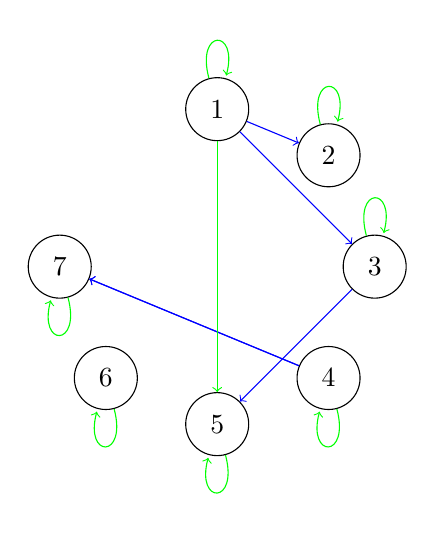
\begin{tikzpicture}[, every node/.style={circle, draw, minimum size=8mm}]
            % Nodes
            \node (1) at (90:2) {1};
            \node (2) at (45:2) {2};
            \node (3) at (0:2) {3};
            \node (4) at (-45:2) {4};
            \node (5) at (-90:2) {5};
            \node (6) at (-135:2) {6};
            \node (7) at (180:2) {7};

            %self loop
            \foreach \i in {1,...,3} {
                \draw[->,green] (\i) edge [loop above] (\i);
            }
            \foreach \i in {4,...,7} {
                \draw[->,green] (\i) edge [loop below] (\i);
            }

            % Edges
            \draw[->,blue] (1) -- (2);
            \draw[->,blue] (1) -- (3);
            \draw[->,blue] (3) -- (5);
            \draw[->,blue] (4) -- (7);
            \draw[->,blue] (4) -- (7);
            \draw[->,green] (1) -- (5);
        \end{tikzpicture}
        \caption{First model}
    \end{minipage}
    \quad
    \begin{minipage}[b]{0.45\linewidth}
        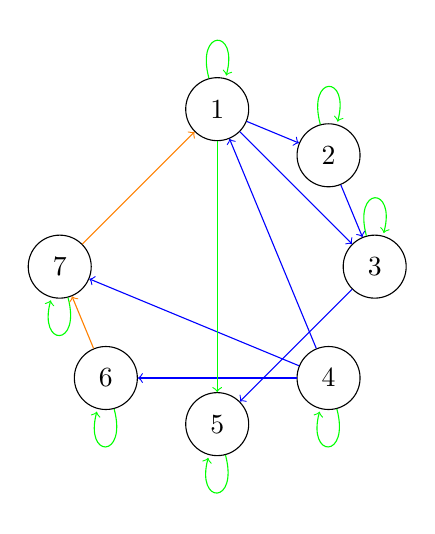
\begin{tikzpicture}[, every node/.style={circle, draw, minimum size=8mm}]
            % Nodes
            \node (1) at (90:2) {1};
            \node (2) at (45:2) {2};
            \node (3) at (0:2) {3};
            \node (4) at (-45:2) {4};
            \node (5) at (-90:2) {5};
            \node (6) at (-135:2) {6};
            \node (7) at (180:2) {7};

            %self loop
            \foreach \i in {1,...,3} {
                \draw[->,green] (\i) edge [loop above] (\i);
            }
            \foreach \i in {4,...,7} {
                \draw[->,green] (\i) edge [loop below] (\i);
            }

            % Edges
            \draw[->,blue] (1) -- (2);
            \draw[->,blue] (1) -- (3);
            \draw[->,blue] (3) -- (5);
            \draw[->,blue] (4) -- (6);
            \draw[->,blue] (4) -- (7);
            \draw[->,blue] (2) -- (3);
            \draw[->,green] (1) -- (5);
            \draw[->, orange] (6) -- (7);
            \draw[->, orange] (7) -- (1);
            \draw[->,blue] (4) -- (1);
        \end{tikzpicture}
        \caption{Second model}
    \end{minipage}
    \end{figure}
    
    The first model expresses $T$ as the reflexive transitive closure of the input $E$, whereas the second model expands the first model and adds more additional atoms to a model.
\end{contexample}

Such an ambiguity is not ideal when we want to compute the query results of datalog. Some fragments of logic programming allow multiple models such as answer-set programming, but for datalog, we want a unique model. This is known as the least model. For this, we need to define what least means and show that it exists.

We call a set of ground atoms an \textit{interpretation}. An interpretation represents all true atoms. We want to define the model property from first-order logic for this definition and show then that there exists a least model according to the subset relation.

Recall from first-order logic that $\forall x. \phi(x)$ holds in a structure $\mathcal{A}$ if any element $a \in \mathcal{A}$ we have that $\phi(a)$ holds. As we do not have any function symbols all elements in the universe are constants, so instead of using the universal quantifier we could just create rules by replacing variables with all possible constants.
Formally, this is defined using \textit{groundings} or \textit{instantions} which are functions that map variables to constants. We can apply a grounding $g$ to an atom by replacing every variable $v$ in the terms by $g(v)$ and apply $g$ to a rule by applying it to the head and every atom in the body. At the end of this, we have replaced every variable by a constant and have gained a ground rule. 
The ground program $ground(P)$ of a program $P$ is the set of all ground rules that are the result of applying some grounding to a rule from $P$

We call a ground rule $r$ \textit{true} in an interpretation $I$ if whenever $Body(r)$ is a subset of $I$, then also $Head(r)$ is in $I$.  We call an interpretation $I$ a \textit{model} of a program $P$ if every rule of $ground(P)$ is true in $I$.

So now we have defined models and can define the least model as well. We still need to show that the least model exists for which the following lemma is helpful.

\begin{fact}\label{fact:ModelIntersection}
Let $M_1, M_2$ be two models of a program $P$. Then also $M_1 \cap M_2$ is a model of $P$.
\end{fact}

Therefore the intersection of all models is a model as well and due to the properties of the intersection it is least according to the subset relation. 

In total, we call \[\bigcap_{\text{$M$ is model of $P$}} M\] the \textit{least model} of $P$ and refer to this characterization as the \textit{model-theoretic semantics} of $P$.

\begin{contexample}
    In this example, the first model is actually the least model and the second model is just some other model.

    Therefore the semantic of this program is whenever $Q()$ is given, the reflexive-transitive closure of $E$. 
    If $Q()$ is not given then it is only the reflexive closure.

    Additionally, we see that the rules for $T$ encode general rules whereas the other rules are more a specific input. We might want to reuse these rules for many different instances of $E$, but so far we also need to write a new program.
\end{contexample}

The example raises questions about the reusability of a program. Additionally, we talked in the introduction about database queries but never talked about databases. 

We consider a \textit{database} as a set of ground atoms similar to an interpretation. What is now the semantics of a program $P$ and a database $d$? We simply add every element of $d$ as a fact to $P$ and reuse the previous semantics. Additionally, we can also move all the specific facts from the program into the database and gain a reusable program.
An alternative model definition for a pair of $P$ and $d$ is therefore: An interpretation $I$ is a model for $P$ and $d$ if every ground atom from $d$ is in $I$ and every rule from $ground(P)$ is true in $I$. \cref{fact:ModelIntersection} holds again and we reuse the definition for the database and program case.

Both views are equivalent. We have shown how we can simulate a database by a program. We can simulate the program case with the program and database case by simply using an empty database.

We have now defined the semantics and shown a connection with databases. But this definition is not exactly ideal. In order to find the semantics of a program we would need to check all interpretations and then intersect them all. This is computationally expensive. Is there a simpler way?

We can define a function that computes the least model in a more direct way. For this, we consider the case where only the program $P$ is present.

Consider an interpretation $I$. We call a ground atom $a$ an \textit{immediate consequence} of $I$ if there exists a ground rule $r$ in $ground(P)$ with the head $a$ and $Body(r) \subseteq I$.

The immediate consequence operator $T_P$ adds all immediate consequences to a model. 

\[T_P(I) = \{ a \mid \text {$a$ is an immediate consequence of $I$}\} \]

A fixed point of a function $f$ is an element $k$ such that $f(k) = k$. The repeated application of $T_P$ starting from $\emptyset$ yields a fixed point that is equal to the model-theoretic semantics of a program $P$. 

\begin{contexample}
    We consider again the program $P$. 

    Due to the fact $E(1,3) \leftarrow$, $E(1,3)$ is an immediate consequence of $\emptyset$. Applying $T_P$ again, we have that $T(1,3)$ is an immediate consequence of $\{E(1,3)\}$ due to the rule $T(?x,?y) \leftarrow E(?x, ?y)$ with the grounding 
    
    \[
    g(v) =
    \begin{cases}
        1 & \text{if } v = ?x \\
        3 & \text{else}
    \end{cases}
    \]

    Applying this to every fact, we gain an interpretation $I$ that contains $T(1,3)$ and $T(3,5)$. Then $T(1,5)$ is an immediate consequence of $I$ due to the rule $T(?x, ?z) \leftarrow T(?x,?y) \and T(?y, ?z)$ and the grounding 

    \[
    g'(v) =
    \begin{cases}
        1 & \text{if } v = ?x \\
        3 & \text{if} v = ?y \\
        5 & \text{else}
    \end{cases}
    \]
\end{contexample}

The least fixed-point of $T_P$ is called the \textit{fixed-point semantics} of $P$ and is the basis for most implementations of datalog reasoners. 

Our goal is to explain why an atom is in the datalog result. The third important semantic of datalog helps here. 

A tree $t$ of ground atoms is a proof tree for a ground atom $a$ in a program $P$ and database $d$ if the following three conditions hold:

\begin{enumerate}
    \item the root of $t$ is $a$
    \item for every node $n$ and its children $l$ in $t$ one of the following two conditions holds: 
    \begin{enumerate}
        \item $n \leftarrow l_1 \land ... l_n$ for $l_1,.., l_n \in l$ is a ground rule from $ground(P)$, or
        \item $n$ is a leaf and $n$ is in the database.
    \end{enumerate}
\end{enumerate}

\begin{figure}
    \centering
    \begin{subfigure}[b]{0.45\linewidth}
    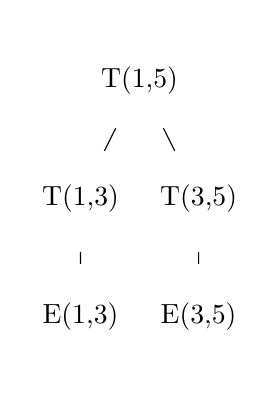
\begin{tikzpicture}[, every node/.style={circle}]
        \node {T(1,5)}
            child {node {T(1,3)}
                child {node {E(1,3)}}
                }
            child {node {T(3,5)}
                child {node {E(3,5)}}};
    \end{tikzpicture}
    \label{prelim:validTree}
    \caption{A valid proof tree}
    \end{subfigure}
    \quad
    \begin{subfigure}[b]{0.45\linewidth}
        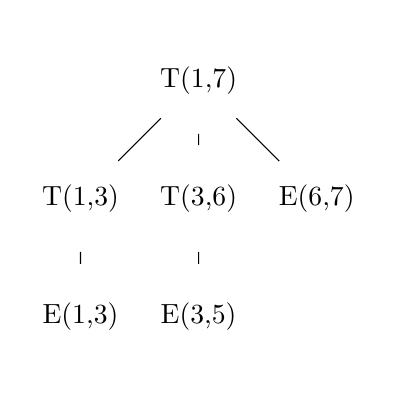
\begin{tikzpicture}[, every node/.style={circle}]
            \node {T(1,7)}
                child {node {T(1,3)}
                    child {node {E(1,3)}}
                    }
                child {node {T(3,6)}
                    child {node {E(3,5)}}}
                child {node {E(6,7)}};
        \end{tikzpicture}
        \caption{An invalid tree}
        \label{prelim:invalidTree}
    \end{subfigure}
    \end{figure}

\begin{contexample}
    The tree in \cref{prelim:validTree} is valid. The leaves of this tree are facts and all other nodes represent ground rules from $ground(P)$ in the previous step.

    The tree in \cref{prelim:invalidTree} is not valid. $E(6,7)$ is neither a fact nor in the database. Additionally there is no rule in $P$ that can result into $T(1,7) \leftarrow T(1,3) \land T(3,6) \land E(6,7)$.
\end{contexample}

The proof-theoretic semantics of a program $P$ and database $d$ is the set of ground atoms that have a valid proof tree. Again this can be shown to be equal to the other semantic definitions. We will formally prove the equality of the proof-theoretic and the model-theoretic semantics of datalog in this work.

In the rules of the program $P$ we note a special rule of the form $T(?x, ?x) \leftarrow$. It is a fact, but not a ground rule and the only rule where this is the case. 
We call a rule $H \leftarrow B_1 \land ... \land B_n$ \textit{safe}, if every variable that occurs in the head also occurs in the body, i.e. \[Vars(H) \subseteq \bigcup_{i \in \{1,..,n\} } Vars(B_i) \]

We call a program safe if every rule in the program is safe. Safe programs are considered better because their result does not depend on the set of constants $C$ which is in practice often either not given or infinite, but only on the specific database and/or the facts in the program.

\begin{contexample}
    We can transform $P$ into the safe program $P'$ by adding a new unary predicate $N$ to the predicate symbols. $P'$ is then the union of $P \setminus \{T(?x, ?x) \leftarrow \}$ and the following rules:
    \begin{equation}
        \begin{split}
            N(?x) &\leftarrow E(?x, ?y) \\
            N(?y) &\leftarrow E(?x, ?y) \\
            T(?x,?x) &\leftarrow N(?x) \\
        \end{split}
    \end{equation}

    The new predicate $N$ (for nodes) represents any elements that occur in the $E$ relation and is used in the body for the reflexive rule.

    If some constants are desired that do not occur in any $E$ relation, one can also directly encode that into the database.
\end{contexample}

What are the semantics of this newly created safe program $P'$? It turns out, that it is equal to the semantics for $P$ for all original predicates, i.e. if we remove all ground atoms that use $N$ we gain the same result. Therefore we state that any program can be transformed into an equivalent safe program.

\subsection{Certifying algorithms}

\begin{figure}
    \centering
    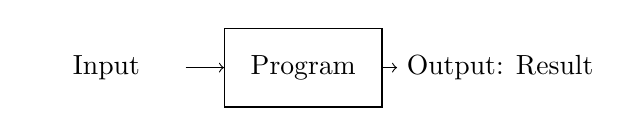
\begin{tikzpicture}[node distance=2.5cm and 20cm, auto]

        \tikzstyle{block} = [rectangle, minimum width=2cm, minimum height=1cm, text centered]
        
        \node [block] (box1) {Input};
        \node [block, right of=box1, draw] (box2) {Program};
        \node [block, right of=box2] (box3) {Output: Result};
        
        \draw [->] (box1.east) -- (box2.west);
        \draw [->] (box2.east) -- (box3.west);
        
    \end{tikzpicture}
    \caption{A convential algorithm}
    \label{fig:programNormal}
\end{figure}

\begin{figure}
    \centering
    \begin{tikzpicture}[node distance=3cm and 3cm, auto]

        \tikzstyle{block} = [rectangle, minimum width=2cm, minimum height=1cm, text centered]
        
        \node [block] (box1) {Input};
        \node [block, right of=box1, draw] (box2) {algorithm};
        \node [block, below of=box3] (box4) {Certificate};
        \node [block, right of=box2] (box3) {Result};
        \node [block, right of=box3, draw ] (box5) {Checker};
        \node [block, right of=box5 ] (box6) {Accept/Not accept};
        \node [block, above of= box6] (box7) {Output};

        \draw [->] (box1.east) -- (box2.west);
        \draw [->] (box2.south) |- (box4.west);
        \draw [->] (box2.east) -- (box3.west);
        \draw [->] (box3.east) -- (box5.west);
        \draw [->] (box4.east) -| (box5.south);
        \draw [->] (box5.east) -- (box6.west); 
        \draw [->] (box3.north) |- (box7.west); 
    \end{tikzpicture}
    \caption{A certifying algorithm algorithm}
    \label{fig:certifyingAlgorithm}
\end{figure}

Most algorithms one encounters either in books like \cite{AlgorithmsBook} or in real programs are comparable to \cref{fig:programNormal}. We have an input, give this into an algorithm which is a black box for us and then we receive a result as an output. Without inspecting the implementation we have to trust that the results are correct.
An alternative to this are \textit{Certifying algorithms} depicted in \cref{fig:certifyingAlgorithm}. They offer an explanation in addition to the result that can be checked independently by the checker or the user themselves. We follow the presentation in \cite{CertAlg} which offers information far beyond this section as well. 

Recall a definition of the class NP from complexity theory:

\begin{definition}[\cite{complexityBook}]
    A language $L \subseteq \{0,1\}^\star$ is in NP if there exists a polynomial $p: \mathbb{N} \to \mathbb{N}$ and a polynomial-time Turing machine $M$ such that forall $x \in \{0,1\}^\star$:

    \[ x \in L  \Leftrightarrow \exists u \in \{0,1\}^{p(|x|)}\text{ s.t. } M(x,u) = 1\]

    If $x \in L$ and $u \in \{0,1\}^{p(|x|)}$ satisfy $M(x,u) = 1$, then we call $u$ a certificate for $x$
\end{definition}

We can generalize this and require an algorithm not only to give us an output $x$ but also a certificate $u$ as a reason why $x$ is the correct output. Then we can either check by ourselves that $x$ is a correct solution according to $u$ or use another program that checks this. As verifying a solution is never harder than computing it, the checker is usually simpler so that we either see directly that the checker is correct or we can formally verify it.

The formal framework of \cite{CertAlg} defines certifying algorithms in the following way. We consider the set $X$ of input values and the set $Y$ of output values of a function $f$. A predicate $\phi: X \to \{true, false\}$ states a precondition for the inputs and another predicate the postcondition $\psi: X \times Y \to \{true, false\}$, $\phi$ allows us the algorithm to only accept part of the input space and $\psi(x,y)$ typically expresses that $y$ is a valid output for the input $x$. In cases where $x$ is not a valid input, we use the new symbol $\bot$ to denote that the algorithm does not return anything and denote by $Y^\bot = Y \cup \{\bot\}$.
The certificate or \textit{witness} from a set $W$ and its correctness is expressed by the predicate $\mathcal{W}: X \times Y^\bot \times W$ with the following properties:

\begin{enumerate}
    \item \textbf{Strong witness property}: Consider a triple $(x,y,w)$ that satisfies the witness predicate $\mathcal{W}$. If $y=\bot$, i.e. the input is not valid, we want $w$ to be a proof of this fact. Else we have that $y\in Y$ and we want $w$ to be a proof that the postcondition is satisfied, i.e.
    \[ \forall x,y,w (y = \bot \land \mathcal{W}(x,y,z) \rightarrow \neg \phi(x)) \land (y \in Y \land \mathcal{W}(x,y,z) \rightarrow \psi(x,y)) \]
    \item \textbf{Simplicity}: This statement above has a simple proof
    \item \textbf{Checkability}: It is possible to check efficiently if $\mathcal{W}(x,y,z)$ holds for a triple $(x,y,z)$
\end{enumerate}

A \textit{(strongly) certifying algorithm} is an algorithm that stops on all inputs $x \in X$ and returns a tuple $\langle y, w\rangle$ such that $\mathcal{W}(x,y,w)$ holds.

This is explained in the following examples. We start with an example from graph theory.

\begin{example}[\cite{CertAlg}]
    Consider the problem of deciding whether a graph $G=(V;E)$ is bipartite, i.e. there exists a partition of $V$ into $V_1, V_2$ with $V = V_1 \cup V_2$ and $V_1 \cap V_2 = \emptyset$, such that for all edges $e \in E$ we have that $e \cap V_1 \neq \emptyset$ and $e \cap V_2 \neq \emptyset$, so that all edges are only between vertices that are in the different partitions.

    The set of inputs $X$ is the set of strings over $\{0,1\}$ and $\phi(x)$ holds whenever $x$ encodes a graph. 
    The postcondition is the following: If $y= true$, then $x$ encodes a bipartite graph. If $y = false$, then $x$ does not encode a bipartite graph.

    Adopting the well-known algorithm for checking whether a bipartite graph, we can construct the following certifying algorithm.

    \begin{enumerate}
        \item Check if $x$ encodes a binary graph. If not return $\bot$ and a witness that describes the problem in the encoding.
        \item Explore the graph in depth-first search and color vertices along the path by alternating colors. If we want to color a vertex by a color $c$ and it already has the color $c'$, we continue exploring another path if $c=c'$, or stop if $c \neq c'$ and return $false$. If that is the case, we have a cycle of odd length in our current path and return this cycle as a witness.
        \item If we reach this step, then all vertices are colored in a way that no neighboring vertices have the same color. Then we return $true$ and the two sets of colored vertices as the witness. 
    \end{enumerate}

    We know from graph theory that a graph is bipartite iff it has no cycle of odd length.

    For any value of $y$ a checker can efficiently check if the returned reason does indeed hold for $x$.
\end{example}

The above example illustrates the example well for a decision problem, but we want to decide whether a set of ground atoms is the semantics of a datalog program and database, i.e. a function problem. The next example illustrates a certifying algorithm for a function problem in number theory.

\begin{example}[\cite{CertAlg}]
    Let $X$ be the set of pairs of natural numbers and $Y$ the set of natural numbers. We want to compute the greatest common divisor, $gcd$, for two numbers $a$ and $b$ that are not equal to zero, i.e. the largest $g \in \mathbb{N}$ that is a divisor of both $a$ and $b$. The precondition $\phi(\langle a, b\rangle)$ is that both $a$ and $b$ are different from zero and $psi(\langle a, b\rangle, g)$ shall me to true, if $g$ is $gcd(a,b)$

    The normal way of computing this involves the Euclidean algorithm, but this is not certifying. The extended Euclidean algorithm however returns in addition to the greatest common divisor $g$ two numbers $s$ and $t$ such that $g = gcd(a,b) = a \dot s + b \dot t$. In \cite{CertAlg}, the back direction is proven, i.e. that if $g$ is a divisor of $a$ and $b$ and $g = a s + b  t$, then $g$ is also the greatest common divisor of $a$ and $b$.

    Therefore a certifying algorithm in order to compute the $gcd$ is the extended euclidean algorithm, that returns as $y$ $gcd(a,b)$ and as the certificate the pair $\langle s, t\rangle$

    A checker then only has to check that $g=a s + b t$ hold and that $g$ divides both $a$ and $b$. 
\end{example}

For decision problems, we require an explanation when the input is in a language as well as an explanation when the input is not in the language. A common misconception is that therefore certifying algorithms are only possible for problems that are known to be in $NP \cap coNP$, which is presumed to not include the interesting $NP$-complete problems. This is not the case as we do not require the certificate to be polynomial in the size of the input. Indeed, SAT-solvers that decide the NP-complete satisfiability problem of propositional logic offer certificates in the DRAT proof format as a model or a proof of unsatisfiability\cite{DRAT}.

In the datalog case, many modern reasoners such as Nemo or Soufflé already offer certificates for atoms in the form of the previously introduced proof trees. We therefore focus on implementing a checker for datalog.

In \cite{CertCheckerWorkflow} an approach to develop checkers for certifying algorithms is outlined. There the checker is implemented in C because already the certifying algorithm itself is written in C++, so that both versions are similar. In order to verify the correctness of the checker they employ the proof assistant Isabelle. The C-code is exported by a tool into Isabelle so that the verification can take place. In Isabelle then the problem is defined and it is proven that the export does fulfill the desired properties. 

In this workflow, we have to trust the correctness of the hardware, the C compiler, the tool that exports C code to Isabelle and of Isabelle itself. Additionally, we have to trust that we have correctly defined and specified the problem in Isabelle.

In this work, we modify this workflow a bit. We use a different proof assistant, Lean, instead of Isabelle. Lean not only a proof assistant but also a functional programming language. Therefore we can implement the checker directly in Lean and do not have to export a model of our code into the proof assistant. Our trust base is therefore smaller, as we no longer need an additional compiler for the language the checker is written in nor a tool to export this into the proof assistant. 


\subsection{Lean}
We introduce in this section Lean, a programming language and proof assistant. As of writing, the current version is Lean 4. A more in-depth introduction can be found in \cite{theoremProvingLean} or \cite{functionalProgrammingLean}.

Lean's core is a small trusted kernel\cite{LeanSysDescr}, that captures the most important functionalities and can be extended by the user. Since version 4 Lean is implemented in Lean itself\cite{Lean4}. The most important libraries for Lean that we will use are the standard library Std4\cite{stdLean} which contains important data structures and tactics and mathlib4\cite{mathlib}, which contains definitions, tactics and theorem from diverse areas of mathematics and computer science.

As we have just heard, Lean can encode many mathematical results. The foundations of mathematics are often built on top of set theory (e.g. \cite{logic}) but most proof assistants instead use \textit{type theory}. Type theory was introduced by Bertrand Russel as an alternative foundation during the foundational crisis of mathematics.

Any element, a \textit{term}, has a \textit{type} in type theory. This is denoted by \lstinline|term:type|. 

\begin{example}
    Different terms in their types are displayed below:
        \begin{lstlisting}
            42:nat
            true:bool
            sort([1,2,3]): List (nat)
            nat: Type
            Type: Type₁
        \end{lstlisting}

        \lstinline|nat| is a natural number, \lstinline|true| is a boolean, the result of the application of \lstinline|sort| to \lstinline|[1,2,3]| has the type \lstinline|List nat|. All previous types have a type as well, \lstinline|Type|. \lstinline|Type| itself also has a type \lstinline|Type₁|. This forms an infinite sequence of \textit{type universes}, that are non-cumulative, i.e. no term has multiple types.
\end{example}


In contrast to set theory, functions are a direct element of type theory and do not need a complicated encoding. For any types \lstinline|A| and \lstinline|B|, there exists the type of functions from A to B, \lstinline| A $\to$ B|.

We can define functions in Lean by the keyword \lstinline|def| similar to other functional programming languages, such as the id function for natural numbers. In the parentheses, we denote an argument \lstinline|x| with its type. Due to currying a function can have multiple arguments. After the colon, we denote the returned type of the function, which is here again a natural number. Therefore we have the following type \lstinline|$\mathbb{N} \to \mathbb{N}$|, as the function takes a natural number as an input and returns a natural number as well. After the \lstinline|:=| we denote the natural number this function returns. 
\begin{lstlisting}
            def id (x: $\mathbb{N}$): $\mathbb{N}$:= x
\end{lstlisting}

Everything we have seen so far holds in general in type theory. Lean itself is based however on a specific type theory, the Calculus of Inductive Constructions (CIC), a dependent type theory\cite{Lean4, CoC}.

The id function we defined above is correct but only works for natural numbers. We would have to implement another id function for booleans, string or any other type. This is rather cumbersome because we never actually use any properties of the specific type. We can generalize this function to help us with this problem.

\begin{lstlisting}
            def id (A: Type)(a: A): A:= a
\end{lstlisting}

This id function has now two arguments. The first argument is the type we want to use it on, the second argument is an element of this type. \lstinline| id $\mathbb{N}$| works as previously and has the type \lstinline|$\mathbb{N} \to \mathbb{N}$|. It seems less clear which type id itself has because this depends on the first argument.
Such types are called \textit{dependent types} and we would denote this specific type as \lstinline|$\Pi$ (A:Type) A $\to$ A|, known as a \textit{Pi type} Intuitively, a Pi type is a function that returns a type for any input value.

In practice, we often do not want to write down too much. We can write the function instead also as:
\begin{lstlisting}
            def id {A: Type}(a: A): A:= a
\end{lstlisting}

Now the type $A$ is an implicit argument, which is denoted by the braces, and Lean can fill it in for the user based on the input $a$. Therefore the user can write just \lstinline|id 42| instead of \lstinline|id $\mathbb{N}$ 42|.

So far we have discussed what types are and how we can define functions that are important for the programming aspect of lean, but this does not tell us much about the use as a proof assistant. Due to the Curry-Howard correspondence a proof of statement can be equivalently seen as a function that has the type of the statement. This type of statements is known in Lean as \lstinline|Prop|. There exist functions like \lstinline|Or: Prop $\to$ Prop $\to$ Prop| and the dependent types form the quantifiers. We view the Pi-type $\Pi (a:A), \beta(a)$ as a function mapping $a$ to the true statements of $\beta(a)$, which is equivalent to the universal quantor. Prop therefore has elements such as \lstinline|$\forall (x:$\mathbb{N}), 0 $\le$ x | or \lstinline| x = y $\lor$ $\neg$ x = y|.

Every statement defines its own type, whose elements are the proofs for it. In contrast to other types, all elements of these types are equivalent which is known as \textit{proof irrelevance}, so that elements of these types only serve as a witness for their truth.

Proofs can be constructed in Lean in two ways.  We start by writing \lstinline|theorem| (or lemma, proposition etc. in mathlib) and denote it as we did for a function. The main difference is that the type is what we want to prove and that the function can not be executed.

\begin{lstlisting}
theorem testTheorem {A: Type}: ∀ (x y z: A), x = y → id y = z → z = x := by
  intro x y z h1 h2
  unfold id at h2
  rw [h1]
  apply Eq.symm
  exact h2
\end{lstlisting}

The proof is done in tactic mode. We open the tactic mode with the keyword \lstinline|by|. At the start our context only contains that $A$ is a type and the goal is $∀ (x y z: A), x = y → id y = z → z = x$, which is compactly written as

\[ \{A:Type\} \vdash ∀ (x y z: A), x = y → id y = z → z = x\]

We apply tactics to change the goal or a hypothesis in the context. These may introduce new goals or fulfill old goals. A proof is finished, when all goals are proven. We explain the proof now in more detail.

\begin{enumerate}
    \item We start with the \lstinline|intro| tactic. This moves elements that are universally quantified or the start of an implication from the goal into the context. Alternatively, one can use \lstinline|revert| to move a hypothesis from the context back to the goal to prove a stronger statement.
    
    At the end, the state is: 

    \[ \{A:Type\} (x y z: A) (h1: x = y) (h2: id y = z)\vdash z = x\]

    \item After that we use the \lstinline|unfold| tactic at the hypothesis h2. This replace \lstinline|id| with its definition in h2, which now looks like this: $(h2: y = z)$
    
    \item We use now the tactic \lstinline|rw|, i.e. rewrite, that replaces in the goal $x$ by $y$ due to the hypothesis $h1$ so that the goal is now $z = y$
    \item The goal is now almost the same as $h2$, but the order is wrong. Therefore we use the apply tactic with
    
    \lstinline|Eq.symm := $\forall \{A:Type\} (a b:A), a = b \rightarrow b = a$ |. 

    Apply tries to match the statements consequent with our goal and opens new goals for the antecedents of this statement.

    Our current proof state is this:

    \[ \{A:Type\} (x y z: A) (h1: x = y) (h2: y = z)\vdash y = z\]

    \item Our goal is now exactly the same as the hypothesis $h2$. The \lstinline|exact| tactic uses $h2$ to complete the goal.
\end{enumerate}

Other important tactics not seen here are \lstinline|by_contra| which allows a proof by contradiction, \lstinline|by_cases| which allows a case distinction or \lstinline|constructor| that splits an and statement into two goals. Lean offers also methods that try to prove goals themselves like \lstinline|simp| that uses lemmas marked with \lstinline|@simp| or \lstinline|tauto|, that can recognize some tautologies. The set of tactics is however not fixed and the user can introduce new tactics to simplify the reasoning process.

The majority of formal proofs in this work are done in tactics mode, but we see above that describing them in natural language is quite verbose. Therefore we will only describe the idea we followed outside of this section.

These proofs are done backwards, i.e. starting from the goal towards the assumptions. There are also forward proofs that start from the assumptions by building hypotheses until we reach the goal or by composing theorems like functions. While this is possible, it was rarely done in this work because. A good source for this is either \cite{theoremProvingLean} or \cite{HitchhikerLogicVer}.

\todo{Tranform the tactic proof into the forward style.}


We can also use \lstinline|def| to define new types. Sets of type \lstinline|A| are in Lean implemented as functions from \lstinline|A| to \lstinline|Prop|. Functions to \lstinline|Prop| are in general not computable so that the membership in a set is also not computable in contrast to for example lists.

\begin{lstlisting}
    def Set (α : Type) := α → Prop
\end{lstlisting}

This introduces a new type. If we want to just use functions that accept contain elements of type \lstinline|Set|, using \lstinline|def| would create a new type for which we would have to define again the set operations $\cup$ or $\cap$. In this case, one can use the \lstinline|abbrev| command which provides a simple alias.

\begin{lstlisting}
    abbrev NatSet := Set $\mathbb{N}$
\end{lstlisting}

The CIC and Lean allow the creation of types by induction. We can create our own implementation of the natural numbers by the \lstinline|inductive| keyword. After that, we list the constructors. These can be constant constructors such as \lstinline|zero| or function creators like \lstinline|succ|
An inductive type may have many constructors of both types or even none as the empty type.

\begin{lstlisting}
    inductive myNat: Type
    | zero: myNat
    | succ: myNat → myNat
\end{lstlisting}

Our definition states that an element of \lstinline|myNat| is either \lstinline|zero| or the result of \lstinline|succ| to some other element of \lstinline|myNat|. Any element of \lstinline|myNat| is only the result of one of these constructors and all elements of \lstinline|myNat| are different.

A typical mathematical definition for this would be: myNat is the smallest set $S$ of elements such that it contains $zero$ and whenever an element $a$ is in $S$, then also $succ(a)$ is in $S$.

We can define for inductive types functions recursively like the add function.

\begin{lstlisting}
    def myNat.add (n m: myNat): myNat :=
    match m with
    | zero => n
    | succ m' => succ (add n m')
\end{lstlisting}

If we want to prove a statement about elements on an inductive type, we can use the \lstinline|induction| tactic to create proofs similar to those by (structural) induction in natural language proofs. If no induction hypothesis is needed one can also use the \lstinline|cases| tactic that creates a goal for every constructor

\begin{lstlisting}
            theorem myNat.add_zero (n: myNat): myNat.add zero n = n := by
                induction n with
                | zero =>
                    unfold add
                    rfl
                | succ n' ih =>
                    unfold add
                    rw [ih]
\end{lstlisting}

We start with the induction tactic to perform an induction over n. Each constructor is listed separately and after the arrow, we start the proof for this constructor. In the zero case, it is enough to unfold the definition of add to get \lstinline|zero=zero| and use \lstinline|rfl| which proves these equalities.

In the succ case, we have two values:  the myNat element $n'$ we use in the constructor of succ and also the induction hypothesis\lstinline|ih: add zero n' = n'|. We can unfold the definition of add again and use \lstinline|rw| to replace \lstinline| add zero n'| by \lstinline|n'| in the goal \lstinline|succ (add zero n') = succ n'|. The \lstinline|rw| tactic applies \lstinline|rfl| at the end automatically to finish the proof.

After defining the natural numbers inductively, we can also define the even numbers by induction. We again have the zero constructor and a succ constructor that now shall represent the next natural number.

\begin{lstlisting}
    inductive evenNat: Type
    | zero: evenNat
    | evenSucc: evenNat → evenNat
\end{lstlisting}

While this works, we see no relation between the elements of myNat and evenNat. We can of course define a function that maps elements of evenNat to myNat and use this to transform any even number to a natural number.

\begin{lstlisting}
    def evenNatToMyNat (e: evenNat) := 
        match e with
        | zero => myNat.zero
        | succ e' => myNat.succ (myNat.succ (evennatToMyNat e'))
\end{lstlisting}

This approach works but is a bit cumbersome. We always need to type this ourselves and if we forget it Lean will complain. There exists however the \lstinline|class Coe|. A class describes an abstract property e.g. of a type and can be implemented by a specific type via \lstinline|instance|.

The \lstinline|Coe| looks (in a simplified version) like this. It takes two types and a function that maps from one type to the other. We can show that this property holds for \lstinline|evenNat| and \lstinline|myNat| by using \lstinline|evenNatToMyNat| to define an instance of this class. Then we can use elements of \lstinline|evenNat| in functions defined for \lstinline|myNat| and Lean will automatically convert them using \lstinline|evenNatToMyNat|.

\begin{lstlisting}
class Coe (α : Type) (β : Type) where
    coe : α → β

instance coeEvenNatMyNat: Coe evenNat myNat := ⟨evenNatToMyNat⟩
\end{lstlisting}

An alternative way of defining types are structures that are comparable to classes in object-oriented languages. Structures have fields that have a type and we start listing them one by one after the \lstinline|where| statement. Structures are like inductive types with a single constructor. Therefore they are not allowed to be recursive, i.e. no structure $A$ may have an element of type $A$, because there would be no base case.
We can build an element of the type of the structure by passing the elements in braces and can use the name of the field to access an element.

\begin{lstlisting}
    structure player where
    (name:String)
    (numGoals: $\mathbb{N}$)
    (active: Bool)

    def player1: player := {
        name := "Test",
        numGoals := 10,
        active := true
    }

    def player1Goals: $\mathbb{N}$ := player1.numGoals
\end{lstlisting}

Returning to our example of myNat, we can define some more functions. In the previous section, we talked about the Euclidean algorithm. We can try to implement it ourselves in Lean. Firstly, we would require the modulo function for that. We will only define it for now to not lose focus and use the keyword \lstinline|sorry| in the value. This closes in proofs any goal or can be used for incomplete functions, but will throw an error if executed.

\begin{lstlisting}
    def myNat.mod (n m: myNat): myNat := sorry
\end{lstlisting}

The Euclidean algorithm can be implemented in the following way:

\begin{lstlisting}
    def myNat.Euclid (a b: myNat): myNat :=
    if b = zero
    then a
    else Euclid b (myNat.mod a b)
\end{lstlisting}

Lean will not accept this function and instead complain in the line of the if that it failed to synthesize an instance of \lstinline|DecidableEq| for myNat. DecidableEq allows us to use $=$ for a type in a function. This is not a trivial requirement as for example the equality of real numbers is undecidable\cite{EqualityRealNumber}. We need to provide a function to Lean that can be used to decide whether two elements of myNat are equal. During the definition of inductive types, we already noted, that all elements of an inductive type are different, which allows us to do this. Luckily, Lean can even do this alone if we tell Lean to do this using the \lstinline|deriving| keyword. It can even derive multiple instances such as the Inhabited instance that states that there exists some default element of this type.

\begin{lstlisting}
    inductive myNat: Type
    | zero: myNat
    | succ: myNat → myNat
    deriving DecidableEq, Inhabited

\end{lstlisting}

Now the error will disappear, but a new one will be introduced. Lean does not recognize the termination of \lstinline|myNat.Euclid|. We have already defined recursive functions before and we did not encounter this problem. In \lstinline|myNat.add| we however used the inductive schema and only did the recursion on $n$ in the case of $succ n$. This allowed Lean to conclude that we only call the function on smaller elements so that the function will terminate.

To show termination, one is required to define some \textit{well-founded relation}, i.e. a relation that does not have any infinite descending chains. Such a relation would be the less-than relation of the natural numbers so it is often convenient to define some size measure that measures the size of our elements in the natural numbers and use this. Such a function exists automatically for any inductive type and is called \lstinline|sizeOf|. We can provide this and are only left to prove that \lstinline|sizeOf (mod a b) < sizeOf b|, which we will leave open here.

\begin{lstlisting}
def myNat.Euclid (a b: myNat): myNat :=
  if b = zero
  then a
  else Euclid b (myNat.mod a b)
termination_by sizeOf b
decreasing_by
  simp_wf
  sorry
\end{lstlisting}

An alternative to this termination proof would be to mark this function using the \lstinline|partial| keyword, which denotes that this function does not always terminate. This is however often not beneficial as we no longer can no longer use the \lstinline|unfold| tactic to gain the definition of this function in a proof.



We want to take a look at another example of an inductive type, that we will often use namely lists. A list (here List' as List is already a standard definition) is either the empty list or the result of combining a list with a new element and we can define a get function

\begin{lstlisting}
    inductive List' (A: Type): Type
    | nil : List' A
    | cons : A → List' A → List' A
    deriving DecidableEq

    def getElement (A: Type) [Inhabited A] (l: List' A): A :=
    match l with
    | nil => Inhabited.default
    | cons hd _ => hd
\end{lstlisting}

We see in this definition a new type of argument. We want to return an element of the list. If the list is empty, this proves to be difficult. In that case, we return the default element that exists because $A$ is an instance of \lstinline|Inhabited|. Such a type-class parameter is given in brackets and Lean will look for the instance when using this function.

This may not always be the desired behaviour and maybe we want to return nothing if the list is empty. In this case, we can use the \lstinline|Option| Type. It has two constructors, one that contains the element and the other symbolizes that there is nothing. Here $\alpha$ has the type \lstinline|Type u| that symbolizes it works for any type universe.

\begin{lstlisting}
    inductive Option (α : Type u) where
    | none : Option α
    | some (val : α) : Option α
\end{lstlisting}

We will also often use the Exception type. This is uses two types and returns one in the error case and the other in the normal case.

\begin{lstlisting}
    inductive Except (ε : Type u) (α : Type v) where
  | error : ε → Except ε α
  | ok    : α → Except ε α
\end{lstlisting}

\begin{figure}
    \centering
    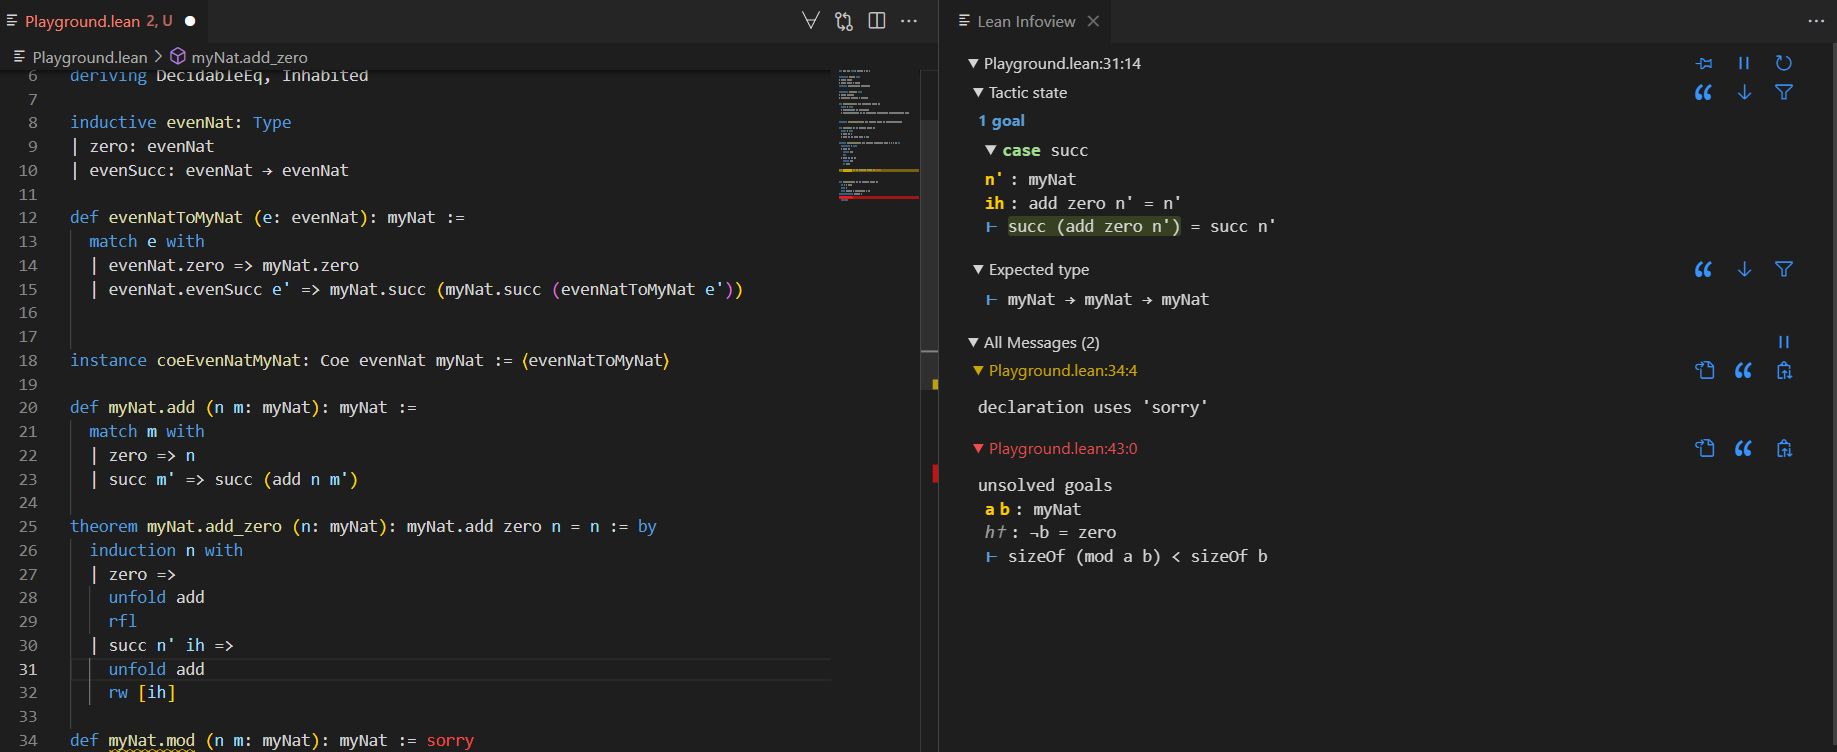
\includegraphics[scale=0.4]{Lean_example.png}
    \caption{An example of Lean in practice. On the left side is the code seen and on the right side the context in a proof with the current goal}
\end{figure}

    \section{Datalog in Lean}
        
        We introduced Datalog in the previous chapter. Here we show our implementation in Lean which we will use later to show the correctness of our algorithms.

        We started defining datalog using sets for constants, variables and relation symbols. In order to correctly interprete an 

        \begin{lstlisting}
            structure signature where
                (constants: Type)
                (vars: Type)
                (relationSymbols: Type)
                (relationArity: relationSymbols → ℕ)
        \end{lstlisting}

        We no longer require that the constants and variables are distinct sets as the constructor for terms allows us to identify the type of a term. We will continue to define the other syntactic elements of datalog. The signature unless displayed otherwise will be $\tau$.

        \begin{lstlisting}
            inductive term :
            | constant : τ.constants → term τ
            | variableDL : τ.vars → term τ
            deriving DecidableEq
        \end{lstlisting}

        As we want to use these objects in practical algorithms we need a way to see if two terms are the same to e.g. replace a variable by a constant. We use Leans ability to automatically create a decidable function for equality for our inductive types and structure from the given functions for the equality of the types from the signature. This allows us to use statements like \texttt{a = b} for atoms \texttt{a, b} in the program we describe in the later sections.
    
        For atoms we have to make sure that the amount of terms matches the arity of the relation symbol. Therefore the structure has an additonal element that is a proof of this property. Two atoms are equal if all fields in the structure are equal. Since propositions as this proof are always equal, it is enough to show that the terms and the symbols are equal.

        \begin{lstlisting}
            structure atom where
                (symbol: τ.relationSymbols)
                (atom_terms: List (term τ ))
                (term_length: atom_terms.length = τ.relationArity symbol)
            deriving DecidableEq

            lemma atomEquality (a1 a2: atom τ): 
            a1 = a2 ↔ a1.symbol = a2.symbol ∧ a1.atom_terms = a2.atom_terms 

        \end{lstlisting}

        Rules and programs can be expressed relatively straight forward. For programs we use \texttt{abbrev}, which introduces program as an alias for \texttt{Finset(rule $\tau$)} from \texttt{mathlib},  instead of defining a new type as this allows us to use the common set operations without the need to redefine them.

        \begin{lstlisting}
            structure rule where
                (head: atom τ)
                (body: List (atom τ))
                deriving DecidableEq

            abbrev program := Finset (rule τ)
        \end{lstlisting}

        We have previously introduced ground atoms as atoms whose terms are only constants. There are at least two options to represent them here. Firstly we could define a structure for ground atoms that extends atoms by a predicate that shows that there are only constants present. The second option is to define an entirely new structure similar to atoms but allow only constants instead of terms. The first options show directly that every ground atom is an atom which we would have to establish separately in the second option. The second option allows directly to define the functions on a list of constants instead of having to cast the list of terms of a ground atom directly to a list of constants and allows to use the complete induction schema when defining functions on ground atoms. The second option seemed to offer more advantegous and was therefore chosen.

        \begin{lstlisting}
            structure groundAtom  where
                symbol: τ.relationSymbols
                atom_terms: List (τ.constants )
                term_length: atom_terms.length = τ.relationArity symbol
            deriving DecidableEq
        \end{lstlisting}

        Now we need a function that maps \texttt{groundAtom} back to \texttt{atom}. For this we can map the \texttt{atom\_terms} list in \texttt{groundAtom} with \texttt{term.constant} to term. Additionally we need to show that the \texttt{term\_length} property is preserved. Luckily, this is already proven in mathlib.


        \begin{lstlisting}
            lemma listMapPreservesTermLength (ga: groundAtom τ): 
            (List.map term.constant ga.atom_terms).length = 
             τ.relationArity ga.symbol :=
            by
                rw [List.length_map]
                apply ga.term_length

            def groundAtom.toAtom (ga: groundAtom τ): atom τ:= 
            {
                symbol:=ga.symbol,
                atom_terms:= List.map term.constant ga.atom_terms,
                term_length:= listMapPreservesTermLength ga
            }
        \end{lstlisting}

        Additionally, we need later that two \texttt{groundAtom} are equal iff the result of \texttt{toAtom} is equal. Similarly, we can define ground rules and functions to convert them to rules.

        For now we have only seen 


        We formalize two semantics here. Firstly, we need the proof-theoretic semantics. Proof trees are a good way to show why an element must be in the solution and output already by multiple datalog engines. There is however to the best of our current knowledge no short certificate similar to proof trees to show the absence of elements. In order to show that a solution is complete we need another method. Both the fixed-point and the model-theoretic semantics offer help in this case. Both are the least element of some set (of fixed-point or of models respectively). Therefore it is enough to show that it is a member of this set for the other direction.

        For the semantics we need the concept of the database. We do not want to deal with the implementation details of a database. We consider it as a black box that returns for a ground atom whether it is in the database. It is a function that returns \texttt{Bool}, because we want computable databases.

        \begin{lstlisting}
            class database (τ: signature) 
            [DecidableEq τ.vars] [DecidableEq τ.relationSymbols]
            [DecidableEq τ.constants]:=
            (contains: groundAtom τ → Bool)
        \end{lstlisting}
        

        We start by defining the proof-theoretic semantics. For this we need to formalize trees. The tree is supposed to start from the facts and then expand upwards by the application of rules. As the body of rules is in general unbounded, we also require trees with an unbounded number of children, which we realize via lists.

        \begin{lstlisting}
            inductive tree (A: Type)
            | node: A → List (tree A) → tree A        
        \end{lstlisting}

        In contrast to binary trees, we will need to use functions for lists to define functions on trees. Most interesting function will however need a proof of termination due to this tree model. 
        
        \begin{lstlisting}
            def root: tree A → A
            | tree.node a _ => a

            def children: tree A → List (A)
            | tree.node _ l => List.map root l

            def listMax {A: Type} (f: A → ℕ): List A → ℕ
            | [] => 0
            | (hd::tl) => 
                if f hd > listMax f tl 
                then f hd 
                else listMax f tl

            def height: tree A → ℕ
            | tree.node a l => 
                1 + listMax (fun ⟨x, _h⟩ => height x) l.attach
            termination_by height t => sizeOf t
            decreasing_by
                simp_wf
                apply Nat.lt_trans (m:= sizeOf l)
                apply List.sizeOf_lt_of_mem _h
                simp
        \end{lstlisting}
        
        Height is recursively called on the elements of in the list via the listMax function. Lean can not identify that this terminates so we have to provide a proof of termination. This is done in Lean by providing a well-founded relation that takes part of the input and show that the recursive calls of the function are only on elements that are smaller in this relation. Due to the well-foundedness there are no infinite descending chains and the function must terminate.  We use the \texttt{sizeOf} function that is built in for any inductive type and maps an element to the successor of the sum of the \texttt{sizeOf} values of the elements used in the sucessor. If we show that this always decreases then the function will terminate as the natural numbers are well-founded.

        In contrast to just using the list, we call listMax on \texttt{List.attach} instead. \texttt{List.attach} takes a list $l$ and creates a new list consisting of pairs of the original elements and a proof that the element is in $l$. This proof can be later used when proving termination.

        We have to show a statement of the form $\mathtt{sizeOf} x < 1 + \mathtt{sizeOf} a + \mathtt{sizeOf} l$. We use the transitivity property of the linear order to show this via showing first that $\mathtt{sizeOf} x < \mathtt{sizeOf} l$ and secondly that $\mathtt{sizeOf} l < 1 + \mathtt{sizeOf} a + \mathtt{sizeOf} l$. This second statement is obviously true and can be found by \texttt{simp}. For the first statement we can use the fact that the size of a member of a list is smaller than the size of the list. Due to using \texttt{l.attach} we have a proof for this available and finish the proof.
        This way of proving termination is the standard way we use in this model and will be omitted for further tree functions.

        Proof trees are then trees that have \texttt{groundAtom} as it vertices and we can formulate the validness criteria. There are two cases. If we are at leaf, i.e. the list of children is empty, then we simply check the database. Else there must exist a rule $r$ from the program and a grounding $g$ so that applying $g$ to $r$ matches the rule created from the current node and its children. Additionally all child trees must be valid as well.

        \begin{lstlisting}
            abbrev proofTree' (τ: signature) := tree (groundAtom τ)

            def isValid(P: program τ) (d: database τ) (t: proofTree τ): 
            Prop :=
            match t with
            | proofTree.node a l => 
            ( ∃(r: rule τ) (g:grounding τ), 
                r ∈ P ∧ 
                ruleGrounding r g = groundRuleFromAtoms a (List.map root l)
                ∧ l.attach.All₂ (fun ⟨x, _h⟩ => isValid P d x)) 
            ∨ (l = [] ∧ d.contains a)
        \end{lstlisting}

        The proof-theoretic semantics is then simply the set of ground atoms that are the root of a valid proof tree.

        \begin{lstlisting}
            def proofTheoreticSemantics (P: program τ) (d: database τ): 
            interpretation τ:= 
            {a: groundAtom τ | ∃(t: proofTree τ), root t = a ∧ isValid P d t}
        \end{lstlisting}

        After that we define the model-theoretic semantics. We choose the model-theoretic semantics over the fixed points semantics as we can directly construct the model and do not have to show that a fixed-point exists. Checking them in practice seems to be similar. 

        An interpretation is a set of ground atoms, that may be a model. A model of a program over a database is an interpretation that contains every database element and fulfills every rule. Choosing the database to be a part of the model simplifies grounding later, as there is only one place to check for matches. Additionally, we want to show that both defined semantics are equal. From the definition above one can see that any database element has a valid proof tree and is therefore in the proof-theoretic semantics.

        \begin{lstlisting}
            abbrev interpretation (τ: signature) := Set (groundAtom τ)

            def ruleTrue (r: groundRule τ) (i: interpretation τ): Prop := 
            groundRuleBodySet r ⊆ i → r.head ∈ i

            def model (P: program τ) (d: database τ) (i: interpretation τ):= 
            (∀ (r: groundRule τ), r ∈ groundProgram P → ruleTrue r i) 
            ∧ ∀ (a: groundAtom τ), d.contains a → a ∈ i
        \end{lstlisting}

        The usual way of defining the model-theoretic semantics is via the model intersection property. If we have two models for a datalog program, then their intersection is again a model. Intersecting all models yields therefore the minimal model. In order to use $\bigcap$ in lead we would need to transform the set of models firstly into an indexed set. We instead used the following more simple notion. We know that an element $a$ is a member of $X \cap Y$ iff $a$ is a member of $X$ and a member of $Y$. Consequently, $a$ is a member of $\bigcap_{M \in models(P,d)} M $, if it is a member in all models.

        \begin{lstlisting}
            def modelTheoreticSemantics (P: program τ) (d: database τ):= 
            {a: groundAtom τ | ∀ (i: interpretation τ), model P d i → a ∈ i}
        \end{lstlisting}

        This describes the same set, but does not offer yet the minimal model property, which we still have to prove.

        We start by showing that it is a subset of every model.
        \begin{lstlisting}    
            lemma leastModel (P: program τ) (d: database τ) 
            (i: interpretation τ) (m: model P d i): 
            modelTheoreticSemantics P d ⊆ i :=
            by
                unfold modelTheoreticSemantics
                rw [Set.subset_def]
                intro a
                rw [Set.mem_setOf]
                intro h
                apply h
                apply m
        \end{lstlisting}

        This follows quickly from the definition. We have to show that if some arbitrary ground atom $a$ is in the model-theoretic semantics then it is in $i$ from the subset definition. $a$ is in the model-theoretic semantics, if it is in every interpretation that is a model. Specifically, it must be a member of i, which is a model by assumption.

        While the previous lemma is called leastModel, we still have to show that it is a model.

        \begin{lstlisting}
            lemma modelTheoreticSemanticsIsModel (P: program τ) 
                (d: database τ): 
            model P d (modelTheoreticSemantics P d)
        \end{lstlisting}

        \begin{lemma}
            Let $P$ be a program and $d$ be a database. 
            
            Then the \texttt{modelTheoreticSemantics} of $P$ over $d$ is a model for $P$ over $d$.
        \end{lemma}
        \begin{proof}
            We show that both conditions hold and start by showing that any rule must be rule. Let $r$ be a arbitrary rule the ground program of $P$. Assume that the body of $r$ is a subset of the \texttt{modelTheoreticSemantics}. If not, then the rule is already true since the body is not true.
            We assume for a contradiction that the head of the rule is not in the \texttt{modelTheoreticSemantics}. From the definition we know that there must exists a model $i$, which does not contain the rule head. We do know however that the body is a subset of the \texttt{modelTheoreticSemantics} and therefore also a subset of $i$. Then the rule $r$ would not be true and $i$ would not be a model and we have reached a contradiction.
        \end{proof}

        After defining both semantics we finally want to show that they are equal, i.e. the following theorem.

        \begin{lstlisting}
            theorem SemanticsEquivalence (P: program τ) (d: database τ): 
            proofTheoreticSemantics P d = modelTheoreticSemantics P d 
        \end{lstlisting}

        This is supposed to be done via the anti-symmetric property of the subset relation, i.e. $\forall X,Y. X \subseteq Y \land Y \subseteq X \rightarrow X = Y$.

        First we want to show that the proof-theoretic semantics are a subset of the model-theoretic semantics. We show the bit stronger statement, that all element in the proof-theoretic semantics are in every model. As the model-theoretic semantics are a model, the first direction follows.

        \begin{lemma}
            Let $P$ be a program, $d$ be a database and $i$ a model of $P$ over $d$. 
            Then \texttt{proofTheoreticSemantics P d} is a subset of $i$
        \end{lemma}
        \begin{proof}
            We want to show that every ground atom in \texttt{proofTheoreticSemantics P d} is also in $i$. A ground atom $a$ is in the proof-theoretic semantics if there exists a valid proof tree that has the root $a$, so that we can instead prove that the root of any valid proof tree $t$ is in $i$.

            We do this using strong induction on the height of $t$ for arbitrary valid proof trees $t$.
            There are two possiblities for valid proof trees. The first is that it only contains the root, which is a database element. As any model must contain the database, the root of this tree must be in $i$.

            The second possiblity is that the root of $t$ and the direct children of the root represent a ground rule $r$ of $P$. In this case all subtrees must be valid as well and have from the definition of the height of a tree a smaller height. Therefore we can apply the induction hypothesis and conclude that the root for all direct subtrees of $t$ is in $i$. This set is however exactly the body of $r$. Since $i$ is a model and $r$ is a rule from $ground(P)$ whose body is already in $i$, the head of of this rule must be in $i$ as well. The head of $r$ is exactly the root of $t$ which finishes the proof.
        \end{proof}

        For the second direction, we need to show that the \texttt{modelTheoreticSemantics} is a subset of the \texttt{proofTheoreticSemantics}. As we know that the model-theoretic semantic is the least model it suffices to show that the proof-theoretic semantic is a model as well.

        \begin{lemma}
            Let $P$ be a program and $d$ a database.

            Then \texttt{proofTheoreticSemantics P d} is a model.
        \end{lemma}
        \begin{proof}
            We have to show that the conditions for a model hold.

            Firstly, that the database is a subset of the proof-theoretic semantics. For every ground atom in the database we can construct a tree with no children that has only this element as the node. This is valid and has the database element as its head, so that the condition is fulfilled.

            Secondly, we have to show that every rule is fulfilled. Let $r$ be a ground rule from $ground(P)$ and assume that the body of $r$ is a subset of proof-theoretic semantics of $P$ over $d$. Then we have to show that $head(r)$ is also in the proof-theoretic semantics of $P$ over $d$. We do this by constructing a proof for $head(r)$. In order to do we require a list $l$ of valid proof trees such that mapping this list with root yields $body(r)$. Then we can create the new proof tree with the node $head(r)$ and the children $l$. This proof tree is valid as all trees in $l$ are valid and $head(r)$ and $l$ are the rule grounding of some rule $r' \in P$. Since $r$ is a ground rule from $ground(P)$ , such $r'$ and grounding $g$ must exists.

            Finally, we have to show that such a list $l$ really exists. We do this by proving the more general lemma.

            \begin{lemma}
                Let $A$ and $B$ be two types. Let $l'$ be a list of type $B$ and $f$ be a function of $A \to B$ and $valid$ be a function from $B$ to $Prop$. Let $S$ be a finite set such that every member of $l'$ is a member of $S$. Additionally, for any $a$ in $S$ exists a valid $b$ with $f(b) = a$. Then exists a list $l$ with mapping $f$ on $l$ yields $l'$ and that all members of $l$ are valid.
            \end{lemma}
            \begin{proof}
                We proof this by induction on $l'$.
                If $l'$ is the empty list, then we use again the empty list. Any member of the empty list is valid and the mapping condition holds as well, because the empty list is mapped to the empty list.

                Now we consider $l'$ to be of the form $hd::tl$. Since $hd$ is a member of $l'$, it is also a member of $S$ and therefore a valid element $hd_b$ exists with $f(hd_b) = hd$. For $tl$ we aquire such a list $tl_b$ from the induction hypothesis, since any member of $tl$ is a member of $l'$ and by that a member of $S$. Then $hd_b::tl_b$ is the required list.
            \end{proof}

            Letting $l'$ be the body of $r$ and $S$ be the finite set consisting of the members of $l$, we fulfill the first requirement. We set $f$ as the root function and $valid$ as $fun t => isValid P d t$. Then by assumption for any element $a$ of $S$ a valid proof tree with the root $a$ exists, since $body(r)$ is already in \texttt{proofTheoreticSemantics P d}. The lemma then presents us the required list of valid proof trees for the body.
        \end{proof}

        


    \section{Soundness}
        After introducing the problem and modelling in Lean, we now describe the algorithm to verify a solution. In this chapter we deal with the soundness, which means here that every atom in the interpretation is actually in the semantics. For this we use the proof trees as the certificate and the proof theoretic semantics.

        A ground atom is in the proof theoretic semantics if there exists a valid proof tree, that has this ground atom as its head. We were provided with all the proof trees and checking the heads is rather easy, so what remains to be checked is the validness of a proof tree, that was defined in the previous chapter.

        \begin{lstlisting}
            def isValid(P: program τ) (d: database τ) (t: proofTree τ): 
            Prop :=
            match t with
            | proofTree.node a l => 
            ( ∃(r: rule τ) (g:grounding τ), 
                r ∈ P ∧ 
                ruleGrounding r g = groundRuleFromAtoms a (List.map root l)
                ∧ l.attach.All₂ (fun ⟨x, _h⟩ => isValid P d x)) 
            ∨ (l = [] ∧ d.contains a)
        \end{lstlisting}

        The second part of this disjunction consists of a database check and an easy check of list emptyness. The first part is more interesting. Since we use there existential quantifiers, we have to implement something to check this. As the program is given as a list of rules, we can simply iterate over this list. For the grounding we however can something more sophisticated, but groundings are not our object of choice for that.

        
        \subsection{Substitutions}
            A grounding is function from variables to constants. This mean that we always need to specify for every variable a constant that it is mapped to. This was good in the definitions to ensure that we always get a ground atom, but raises in the unification case problems as the following example demonstrates.

            \begin{example}
                Consider the signature consisting of $C = \{a,b,c\}$, $V = \{x,y,z \}$ and $R = \{R\}$. Suppose we want to match a list of terms with a list of constant. The first term is $t_1 = x$ and the first constant is $a$. We might use the the grounding $g = x \mapsto a, y \mapsto a, z \mapsto a$.

                Now we want to use this result and match another term $t_2 = y$ with the constant $b$. The variable $y$ is already mapped to a different constant, but we cannot say whether this is due to a previous matching process or simply because we needed to define a value for every input.
                

                
            \end{example}

            Instead, we want to use substitutions that were already introduced in \cite{datalogCoq}. A substitution is a partial mapping from variables to constants. We implement this by mapping to an Option of constant.

            \begin{lstlisting}
            def substitution (τ: signature):= τ.vars → Option (τ.constants)
            \end{lstlisting}

            This allows us to only specify what is necessary. If we apply a substitution to a term, we only replace a variable by a constant, if the substitution is defined for this variable and the constant will be the result of the substitution in this case.

            \begin{lstlisting}
            def applySubstitutionTerm (s: substitution τ) (t: term τ): term τ :=
            match t with
            | term.constant c => term.constant c
            | term.variableDL v => 
                if p: Option.isSome (s v) 
                then term.constant (Option.get (s v) p) 
                else term.variableDL v
            \end{lstlisting}

            We can use similar defintions as previously for groundings to apply substitutions to atoms or rules.

            The main result we want to prove is the following.

            \begin{lstlisting}
            theorem groundingSubstitutionEquivalence 
                [Nonempty τ.constants] (r: groundRule τ) (r': rule τ):
                (∃ (g: grounding τ), ruleGrounding r' g = r) ↔ 
                (∃ (s: substitution τ), applySubstitutionRule s r'= r)
            \end{lstlisting}

            This allows us to replace the grounding check by a substitution check, when trying to validate trees and by this we can bypass the problems that were illustrated in the example above. 

            For the forward implication, we can transform any grounding in a simple way to a substitution. In this substitution every value is defined with the value of the grounding.

            \begin{lstlisting}
            def groundingToSubstitution (g: grounding τ): substitution τ
             := fun x => Option.some (g x)
            \end{lstlisting}

            It is very easy to prove that this is equivalent on every rule.

            For the back direction, we need additionally that the set of constants is non-empty. We can ensure this during the input phase by adding a fresh constant symbol to the constant symbols similar to Herbrand universes. This symbol does not appear in any proof trees and does not influence the results. Since we only look at safe programs, it will also not introduce any new ground atoms to the model.

            The following example shows the problems that occur without the non-emptyness assured.

            \begin{example}
                Consider the program $P= \{p \leftarrow, q \leftarrow p\}$ and the signature $C = \emptyset$, $V = \{x,y,z \}$ and $R = \{p,q\}$

                Any rule in $P$ is already a ground rule and there exists a substitution, the empty substitution that maps all variables to none, so that the rule is equal to itself as a ground rule.
                
                There is however no grounding that can achieve this. We cannot define a grounding since we have no constant available, but have variables that need to be mapped somewhere. Therefore the equivalence does not hold here.
            \end{example}

            Since the set of constants is non-empty, we can use the axiom of choice to get values for which the substitution is not defined.

            \begin{lstlisting}
            noncomputable def substitutionToGrounding 
             [ex: Nonempty τ.constants] (s: substitution τ): grounding τ := 
             fun x =>    if p:Option.isSome (s x) 
                        then Option.get (s x) p 
                        else Classical.choice ex

            \end{lstlisting}

            When introducing substitutions, we had the goal to only add what is needed to a substitution and usually we want the smallest possible substitution. In order to formalize this, we want to define a linear relation on substitutions, that is denoted by $\subseteq$

            Firstly, we define the substitution domain of a substitution as the set of variables for which the substitution is defined. 

            \begin{lstlisting}
            def substitution_domain (s: substitution τ): Set (τ.vars) := 
                {v | Option.isSome (s v) = true}
            \end{lstlisting}

            A substitution $s_1$ is then a subset of a substitution $s_2$, if both substitutions agree on the substitution domain of $s_1$. Outside of this $s_1$ is never defined, whereas $s_2$ might be, so that we view $s_1$ as smaller.

            \begin{lstlisting}
            def substitution_subs (s1 s2: substitution τ): Prop :=
            ∀ (v: τ.vars), v ∈ substitution_domain s1 → s1 v = s2 v
            \end{lstlisting}

            This can be proven to be a partial order.

        \subsection{Unification}

        We know that instead of finding a grounding, it suffices to find a substitution. Now we want to describe an algorithm that tells us whether the ground rule that is formed from a node of the proof tree is the substituted rule of some rule of the program. For this we take inspiration from the unification problem of first-order logic.

        In the unification problem we are given a set of equations between first-order terms and are required to present the most-general unifier.

        Our problem is similar. The equations will not be between terms, but between an object and a ground object of the same corrosponding type and we require a substitution that solves all equations and is minimal in our subset relation.

        An algorithm to solve the first-order unfication problem is the algorithm of Martelli and Montanari \cite{MartMont} and is depicted below:
        \begin{algorithm}
            \caption{Algorithm of Martelli and Montanari}
        \begin{algorithmic}
            \While {There exists some equation for which a transformation is possible}
            \State Pick this equation $e$ and do one of the following steps if applicable
            \begin{enumerate}
                \item If $e$ is of the form $t = t$, then delete this equation from the set.
                \item If $e$ is of the form $f(t_1, .., t_n) = f(s_1,.., s_n)$, then delete $e$ and add $n$ new equations of the form $t_i = s_i$
                \item If $e$ is of the form $f(t_1, .., t_n) = g(s_1,.., s_m)$ with $g \neq f$, then stop and reject.
                \item If $e$ is of the form $f(t_1,..,t_n) = x$ for a variable $x$ and delete $e$ and add an equation with the swapped order to the set
                \item If $e$ is of the form $x=t$ for some variable $x$, then check if x occurs in t. If it does, then stop and reject. If not map all $x$ to $t$ in the set.
            \end{enumerate}
            \EndWhile
        \end{algorithmic}
        \end{algorithm}

        This algorithm offers a good starting point for our own algorithm, but we certain transformation can't occur in the limited syntactic form we operate in. Additionally, we want to output a substitution instead of just answering whether a substitution exists. It is sufficient to do it here, but will later be important. Instead of mapping all $x$ to $t$ as done there in step 5, we will add $x\mapsto t$ to a substitution that is presented as an input. If a variable occurs on the left side, we will check whether it is already in the domain of the substitution and if so check if its current value is consistent with the right side.
        As function symbols appart from constant symbols are not allowed, we can simplify steps 2 and 3, as we never add new equations and instead only check if the constant symbol matches. Finally, as the one side of the equation is always a ground object there will never be a variable on this side, so that we do not have to swap the equation as in step 4.

        We will start with matching a term to a constant with the following algorithm.

        \begin{lstlisting}
            def matchTerm (t: term τ)(c: τ.constants) (s: substitution τ):
            Option (substitution τ) :=
            match t with
            | term.constant c' =>
                if c = c'
                then Option.some s
                else Option.none
            | term.variableDL v =>
                if p:Option.isSome (s v)
                then  if Option.get (s v) p = c
                    then
                        Option.some s
                    else
                        Option.none
                else extend s v c
        \end{lstlisting}

        We are given a term $t$, a constant $c$ and a current substitution $s$ and want to return the minimal substitution $s'$ so that $s \subseteq s'$ and applying $s'$ to $t$ will make it equal to $c$ or none if no such $s'$ exists.

        This is done by case distinction. If $t$ is a constant, then we either return $s$ if $t$ is equal to $c$, or return none as two different constants can not be unified by a substitution. If $t$ is variable, we check if $t$ is in the domain of $s$. If it is already defined we check if the value matches the required value. If it is not defined we extend $s$ with the new mapping $v \mapsto c$.
        Formally extend is defined in the following way:

        \begin{lstlisting}
            def extend (s: substitution τ) (v: τ.vars) (c: τ.constants) :
                substitution τ 
            := fun x => if x = v then Option.some c else s x
        \end{lstlisting}

        We know formally prove the correctness of this algorithm. The first result is that if \texttt{matchTerm} returns a substitution $s'$ that $s'$ is indeed a solution, i.e. that applying $s'$ to $t$ results in $c$ and that $s'$ is an extension of $s$

        \begin{lstlisting}
            lemma matchTermFindsSolution (t: term τ) (c: τ.constants) 
            (s: substitution τ) (h: Option.isSome (matchTerm t c s)): 

            applySubstitutionTerm (Option.get (matchTerm t c s) h) t = c 
            ∧ s ⊆ (Option.get (matchTerm t c s) h)
        \end{lstlisting}
        \begin{proof}
        The proof is done via case distinction. Suppose firstly that $t$ is a constant $c'$. Since matchTerm returned a substitution we must have that $c$ and $c'$ are the same constant and therefore $s'$ is $s$. Applying a substitution to a constant does not change it, so $s' t = s' (c') = c' = c$. Additionally since $\subseteq$ is a linear order and $s' = s$, we have that $s \subseteq s'$

        Now we assume that $t$ is a variable $v$. Now we do another case distinction on whether $s v$ is defined or not. If it is defined, $v$ must already be mapped to $c$ and we return $s$ as this is a solution as seen previously. If it would be mapped to something else, then matchTerm would return none, which would be in violation to our assumptions.
        If it is not defined, we use extend. After that $v$ is mapped to $c$, so that $s' t$ will be equal to $c$. Now we finally have to show that $s \subseteq$ extend $s$ $v$ $c$. We only change the value of $v$. Since $v$ was not defined earlier, for any variable in the domain of $s$, $s$ and extend $s$ $v$ $c$, so that it is fulfilled.
        \end{proof}

        We have proven so far the matchTerm returns a solution, but it might not be a minimal solution. When we want to match atoms with ground atoms, we need to match a list of terms with a list of constants. There it is important that the returned substitution is indeed minimal to conclude whether a solution exists as the following example shows.

        \begin{example}
            Consider the list of terms $l_1 = [x, y, x]$ with the variables $x$ and $y$ and the list of constants $l_2 = [a,b, c]$. We want to find a substitution that we can apply to $l_1$ to gain $l_2$ if possible. We start with the empty substitution and first want to match the first elements of $l_1$ and $l_2$. If we receive a solution $s$, then we continue with the next elements of $l_1$ and $l_2$, but this time the matching extends $s$ instead of the empty substitution.

            Now suppose the procedure $P_1(t,c, s)$ that takes a term, a constant and a substitution does not always return a minimal solution. So it might return for $x$, $a$ and the empty substitution the substitution $s = x \mapsto a, y\mapsto a$.

            Now we again call $P_1$ with $y$, $b$ and $s$. $P_1$ will not return anything, because $y$ is already mapped to something else. From this fact we cannot conclude that there exists no solution at all however. In fact, the non-minimality of the results of $P_1$ prevents this reasoning.

            If we have a second procedure $P_2(t,c, s)$ that always returns the minimal solution we solve the matching process for the first two list elements of each list to return $s' = x \mapsto a, y \mapsto y$. Now we want to match $x$ with $c$ and $P_2$ will return none. We can conclude that no solution exists since any substitution from $P_2$ is minimal. If there exists a solution to the list then $l_2$, it necessarily must match the first to elements of both lists. Since $s'$ is the minimal solution of a process that started with the empty substitution and always returned minimal solution, any solution to the list must extend $s'$. Therefore it must agree on the domain of $s'$ and therefore it must map $x$ to $a$ and therefore no solution can exist.

        \end{example}

        \begin{lstlisting}
            lemma matchTermFindsMinimalSolution' (t: term τ) 
            (c: τ.constants) (s: substitution τ) 
            (h: Option.isSome (matchTerm t c s)): 
            
            ∀ (s': substitution τ),(s ⊆ s' ∧ applySubstitutionTerm s' t = c)
             → (Option.get (matchTerm t c s) h) ⊆ s' :=
        \end{lstlisting}
        \begin{proof}
        This is again done via case distinction on the type of $t$. If $t$ is constant, then $s'$ must be equal to $s$. For any $s^\ast$ with $s \subseteq s^\ast \land s^\ast t = c$ we have b that $s' \subseteq s^\ast$ by the assumption of the property of $s^\ast$

        Now we consider the case of $t$ being a variable $v$ and do a case distinction whether $s v$ is defined. If it was already defined, then $s'$ must again be equal to $s$, so that the claim is fulfilled by the argument above.
        If $s v$ was not defined, we have to show that extend $s$ $v$ $c$ is a subset of any such $s^\ast$. We assume for a contradiction that this is not the case. Then there must be a variable in the domain of extend $s$ $v$ $c$ such that extend $s$ $v$ $c$ and $s^\ast$ differ. Suppose this variable is $v$. Then $s^\ast$ would either not be defined for $v$ or map $v$ to some other constant $c'$. In both cases $s^\ast v \neq c$, so that $s^\ast$ would not be a solution and we would have reached a contradiction.
        If it is some other variable $v'$, then the value of extend $s$ $v$ $c$ is simply the value of $s$. Since $s^\ast$ maps $v$ to a different value compared $s$, $s$ would not be a subset of $s^\ast$ and we have reached another contradiction.
        \end{proof}

        So we know that if matchTerm returns a substitution then it is a minimal solution. We additionally have to prove that if matchTerm does not return a substitution that then no solution exists.

        \begin{lstlisting}
            lemma matchTermNoneImpNoSolution (t: term τ)
             (c: τ.constants) (s: substitution τ)
              (h: Option.isNone (matchTerm t c s)):
            
            ¬ (∃(s': substitution τ), s ⊆ s'∧applySubstitutionTerm s' t = c)
        \end{lstlisting}
        \begin{proof}
        This is again done via case distinction on the type of $t$. If $t$ is a constant $c'$, then $c'$ must be different from $c$, so that matchTerm returns none. Then no substitution can map $t$ to c.

        If $t$ is a variable $v$, then $s v$ must be defined and mapped to a different value compared to $c$. Then again no such $s'$ can exist. If $s$ would be a subset of $s'$, then $s'$ would not unify $t$ with $c$ and if $s'$ would unify $t$ with $c$ then $s$ would not be a subset of $s'$.
        \end{proof}

        After proving the correctness for terms we now want to move up to atoms. Unfortunately, we cannot use recursion directly on the term list of an atom. An atom requires a proof that the length of the list is equal to the arity of the relation symbol, which fails when we do recursion on the list. Therefore we first establish a new procedure that matches a list of terms with a list of constants, if possible.
        
        \begin{lstlisting}
            def matchTermList (s: substitution τ) (l1: List (term τ))
             (l2: List (τ.constants)): Option (substitution τ) :=
            match l1 with
            | List.nil => some s
            | List.cons hd tl =>
                match l2 with
                | List.nil => none
                | List.cons hd' tl' =>
                let s' := matchTerm hd hd' s
                if p: Option.isSome s'
                then matchTermList (Option.get s' p) tl tl'
                else none
        \end{lstlisting}

        Here we are given as previously a substitution as an input with the two lists. For the correctness it is required that both lists have the same length, but this is the case for atoms. If the first list is empty we return the substitution. If instead it has a first element and the second list has as well a first element, we match these elements using matchTerm and if this results in a solution, we return the result of matchTermList with the remaining lists and the resulting substitution.

        As previously, we have to prove the correctness of this algorithm. We again want to show that the algorithm returns the minimal solution iff it exists. We require for these results that both lists are the same length. If the list of constants is longer than the list of terms, the \texttt{matchTermList} function may return a solution eventhough the lists will never be equal. As we only want to use this to match atoms, this is however not a problem. No subsititution can change the symbol, so that we will only try to match atoms with ground atoms that have the same symbol. The symbol determines the number of terms so that both lists will have the same length.

        \begin{lstlisting}
            lemma matchTermListFindsSolution (s: substitution τ)
            (l1: List (term τ)) (l2: List (τ.constants))
            (len: l1.length = l2.length)
            (h:Option.isSome (matchTermList s l1 l2)):
             List.map (applySubstitutionTerm (Option.get (matchTermList s l1 l2) h)) l1 
                = List.map term.constant l2 
             ∧ s ⊆ (Option.get (matchTermList s l1 l2) h ) :=
        \end{lstlisting}
        \begin{proof}
            We prove this by induction on $l_1$ for arbitrary $s$ and $l_2$.
            In the base case $l_1$ is the empty list. Since both lists have the same length $l_2$ must also be the empty list. matchTermList then returns $s$. Applying this to an empty list returns an empty list. Therefore the base case is complete.

            In the induction step we have that $l_1$ is of the form $hd::tl$ and we can similarly assume that $l_2$ is of the form $hd'::tl'$ and that $tl$ and $tl'$ have the same length by our assumption. Since matchTermList returned a substitution, matchTerm $hd$ $hd'$ also must return a substitution $s^\ast$.
            We then use this as an input to gain $s'$ from matchTermList $s^\ast$ $tl$ $tl'$. By the induction hypothesis $s^\ast \subseteq s'$ and applying $s'$ to $tl$ results in it being equal to $tl'$. To show that both lists are equal, we just have to show that after applying $s'$ the heads will be equal. We know that applying $s^\ast$ to $hd$ will result in it being equal to $hd'$. Since $s^\ast \subseteq s'$ and our previous result that if a substitution maps a term to a constant then extension of this substitution will also map the term to the same constant, we have this.
            Lastly, we have to show that $s \subseteq s'$. From the correctness proof of matchTerm we know that $s \subseteq s^\ast$ and from the induction hypothesis we know that $s^\ast \subseteq s'$. Since $\subseteq$ is transitive, the result follows.
        \end{proof}

        After proving that it is a solution, we prove that the solution is minimal.

        \begin{lstlisting}
            lemma matchTermListFindsMinimalSolution (s: substitution τ)
            (l1: List (term τ)) (l2: List (τ.constants)) 
            (len: l1.length = l2.length) 
            (h: Option.isSome (matchTermList s l1 l2)):
            ∀ (s': substitution τ), 
             List.map (applySubstitutionTerm s') l1 = List.map term.constant l2
              ∧ s ⊆ s' → (Option.get (matchTermList s l1 l2) h ) ⊆ s' :=
        \end{lstlisting}
        \begin{proof}
            We prove this again via induction on $l_1$ for arbitrary $l_2$ and $s$. If $l_1$ is empty, we return $s$ and the claim is true by assumption.

            In the induction step we have that $l_1$ has the form $hd::tl$ and we can assume that $l_2$ has the form $hd'::tl'$ and that $tl$ and $tl'$ have the same length. Additionally, we know that matchTerm $hd$ $hd'$ s returns a substitution $s^\ast$. From the induction hypothesis we know that matchTermList $s^\ast$ tl tl' $\subseteq \hat{s}$ for any substitution $\hat{s}$ that extends $a^\ast$ and maps $tl$ to $tl'$. Since $s^\ast$ is a minimal solution for $hd$ and $hd'$ and $s^\ast$ only extends it, we know that it is a solution for the whole list. We also know from the minimality of $s^\ast$ that $s \subseteq s^\ast$. From the induction hypothesis, we get that $s^\ast \subseteq \hat{s}$. Transitivity tells us that $s \subseteq \hat{s}$ as 
        \end{proof}

        Finally the negative case that confirms that the return value of none does indeed state that there is no solution.

        \begin{lstlisting}
            lemma matchTermListNoneImplNoSolution (s: substitution τ)
            (l1: List (term τ)) (l2: List (τ.constants))
            (len: l1.length = l2.length) 
            (h: Option.isNone (matchTermList s l1 l2)): 
            ∀ (s': substitution τ), s ⊆ s' →
            ¬  List.map (applySubstitutionTerm s') l1 = List.map term.constant l2 :=
        \end{lstlisting}
        \begin{proof}
            We prove this again via induction on $l_1$ for arbitrary $l_2$ and $s$. If $l_1$ is the empty list, we cannot return none. As the prerequisite is not fulfilled, the statement is correct.

            In the induction step we have that $l_1$ has the form $hd::tl$ and we can assume that $l_2$ has the form $hd'::tl'$ and that $tl$ and $tl'$ have the same length. There are two cases where matchTermList can return none. The first case is when matchTerm $hd$ $hd'$ $s$ returns none. If that is the case there is no $s'$ with $s\subseteq s'$ and applying $s$ to $hd$ will make it equal to $hd'$. Therefore the two lists cannot be equal either and the proof is finished.

            If matchTerm $hd$ $hd'$ $s$ returns a substitution $s^\ast$, then matchTermList $s^\ast$ $tl$ $tl'$ must return none. From the induction hypothesis we know that there is no substitution $s'$ with $s^\ast \subseteq s'$ and applying $s'$ to $tl$ bringing it equal to $tl'$. Since $s^\ast$ is already the minimal solution to match $hd$ with $hd'$ there cannot exist a solution here.
        \end{proof}

        This can be used to create a matchAtom procedure. We are given an atom and a ground atom and check if the symbols are equal. If they are, we also get that their term lists must be equal as the length of the term list is equal to the arity of the relation symbol. The same symbol implies the same length.
        If the symbols are different, we will never unify them.

        \begin{lstlisting}
            def matchAtom (s: substitution τ) (a: atom τ) (ga: groundAtom τ):
            Option (substitution τ) :=
                if a.symbol = ga.symbol
                then
                    matchTermList s a.atom_terms ga.atom_terms
                else none
        \end{lstlisting}

        The correctness proofs follow from the proofs of matchTermList since we already established the same length of both lists from the symbol.

        Now we can create a \texttt{matchAtomList} function similarly to \texttt{matchTermList} and use this to define a \texttt{matchRule} function. We first try match the head of the rule with the head of the ground rule. If this returns a solution, we use this as the start for matching the bodies. If not, we will not find a solution and return none.

        \begin{lstlisting}
            def matchRule (r: rule τ) (gr: groundRule τ):
             Option (substitution τ):=
                let s := matchAtom emptySubstitution r.head gr.head
                if p: Option.isSome s
                then matchAtomList (Option.get s p) r.body gr.body
                else none

        \end{lstlisting}

        We know prove again that if this returns a substitution then this is a solution and if none is return then there is no solution using our previous results. For both these results we assume that both bodies have the same length, but determining the length of a list can be done in the tree validation process.
        We want a statement with the quantifier to combine it with the theorem about the equivalence between groundings and substitutions. We can prove this statement by using the result of \texttt{matchRule} as a witness for the quantifier. For the back direction, we see that this statement implies that a solution exists, which we always find with \texttt{matchRule}

        \begin{lstlisting}
            theorem matchRuleIsSomeIffSolution (r: rule τ) (gr: groundRule τ) 
            (len: r.body.length = gr.body.length): 
            Option.isSome (matchRule r gr) ↔ 
            ∃ (s: substitution τ), applySubstitutionRule s r = gr
        \end{lstlisting}

        We now have a method to replace this quantifier by a computable function and can finally devise the check for tree validation.

        \subsection{Tree validation}

        We have so far introduced introduced substitutions and have shown a way to decide whether a substitution exists that maps a rule to a ground rule. Now we want to finally show a way to validate trees. As the first step we want to find whether a ground rule $gr$ we gain from the tree is in the ground program, i.e. that there exists a grounding $g$ (or from the previous results a substitution $s$) and a rule $r$ from the program $P$, so that applying $g$ to $r$ yields $gr$. We want to use the \texttt{matchRule} function defined earlier for this. This function required that both bodies of the rules to have the same length in order to work properly. Instead of just computing the length we want to do a bit more. We previously noted that substitutions (or groundings) never change the symbol of an atom, so that we do not have to try to match rules whose symbols differ. The symbols of a rule are expressed in the symbol sequence.

        \begin{lstlisting}
            def symbolSequence (r: rule τ): List τ.relationSymbols := 
             r.head.symbol::(List.map atom.symbol r.body)

        \end{lstlisting}

        We can now compare the symbol sequence of a rule and the symbol sequence of a ground rule. If they are equal, we see that the bodies have the same length, since we just map each body element and attached for both the head at the front. If they are however not equal, then no substitution can be applied to the rule so that it will yield the ground rule.

        We can use this to check whether a ground rule $gr$ is in the ground program of $P$ by computing the symbol sequence of $gr$ and comparing it with the symbol sequence of every rule in the program. For those rules where the symbol sequences are equal, we can apply the \texttt{matchRule} function until we find the first matching rule. While this work, we have to iterate in the worst case always over the whole program. Instead we can preprocess the program into a function that returns for a symbol sequence a list of rules with the same symbol sequence.

        \begin{lstlisting}
            def parseProgramToSymbolSequenceMap (P: List (rule τ)) 
            (m: List τ.relationSymbols → List (rule τ)): 
            List τ.relationSymbols → List (rule τ) :=
            match P with
            | [] => m
            | hd::tl =>
                let seq:= symbolSequence hd
                parseProgramToSymbolSequenceMap tl 
                    (fun x => if x = seq then hd::(m x) else m x)
        \end{lstlisting}

        By induction we can prove that any symbol sequence $s$ the result of 
        
        \texttt{parseProgramToSymbolSequenceMap P m} returns a the list consisting of those rules in $P$ whose symbol sequence matches $s$ and those rules that in $m (s)$. If we therefore use a function that maps any symbol sequence to the empty list for m we get exactly the list of rules that match a particular symbol sequence. As only those rules can result into the ground rule $gr$ with the symbol sequence $s$ by applying a grounding $g$, its enough to iterate over those rules. The \texttt{List.any} function does this and returns true as soon \texttt{matchRule} returns a \texttt{some}. The preprocesssing of $P$ is given as a function $m$, so that it only will be done once.  
        
        \begin{lstlisting}
            def checkRuleMatch (m: List τ.relationSymbols → List (rule τ)) 
            (gr: groundRule τ) (ruleToString: rule τ → String)
            : Except String Unit :=
            if List.any (m (symbolSequence gr.toRule)) 
                (fun x => Option.isSome (matchRule x gr)) = true
            then Except.ok ()
            else Except.error ("No match for " ++ ruleToString gr)
        \end{lstlisting}

        If $m$ is the result of \texttt{parseProgramToSymbolSequenceMap} of $P$ and a function that maps anything to the empty list, \texttt{checkRuleMatch} returns ok if and only if there is a rule $r$ in $P$ and a grounding $g$ such that applying $g$ to $r$ results in the ground rule $gr$.

        \begin{lstlisting}
            lemma checkRuleMatchOkIffExistsRuleForGroundRule 
            (m: List τ.relationSymbols → List (rule τ)) (P: List (rule τ)) 
            (gr: groundRule τ) (ruleToString: rule τ → String ) 
            (ssm: m = parseProgramToSymbolSequenceMap P (fun _ => [])): 
            checkRuleMatch m gr ruleToString = Except.ok () 
            ↔ ∃ (r: rule τ) (g:grounding τ),r ∈ P ∧ ruleGrounding r g = gr
        \end{lstlisting}

        In order to start validating we need another helper function. The tree validation function will return an element of type \texttt{Except String Unit}, so that if the tree is invalid an Exception with an error message in a String is thrown. If it is valid, then nothing is return. In order to show that a tree with the root $a$ is valid, we have to show that all direct subtrees of $a$ are valid using the same function. We could use \texttt{List.all (Except.isOk)} and this would return true iff all subtrees are valid. We would however loose the error message. Instead we define the following function, that returns the first error message it finds.

        \begin{lstlisting}
            def List.map_except_unit {A B: Type} (l: List A) 
            (f: A → Except B Unit): Except B Unit :=
            match l with
            | [] => Except.ok ()
            | hd::tl =>
                match f hd with
                | Except.ok () => List.map_except_unit tl f
                | Except.error b => Except.error b
        \end{lstlisting}

        By induction we prove that it returns \texttt{ok ()} iff for all elements in the list $f$ is evaluated to \texttt{ok ()}.

        \begin{lstlisting}
            lemma List.map_except_unitIsUnitIffAll {A B: Type} (l: List A) 
            (f: A → Except B Unit): 
            List.map_except_unit l f = Except.ok () 
            ↔ ∀ (a:A), a ∈ l → f a = Except.ok ()
        \end{lstlisting}

        In order to validate a tree we have to consider two cases. If it has no children, then it is a fact. This fact may be part of the database or it may be a fact in the program. We can detect if the list of children is empty and ask the database whether it contains the root. If that is the case, the tree is valid and we return \texttt{ok ()}. If not, we use \texttt{checkRuleMatch} to find a fact for the root in $P$ and return the result. Since the tree has no children, all children are valid as well.
        If it has children we try to find a rule using \texttt{checkRuleMatch} that matches the current node and its children and if that is the case we check that all children are valid using the \texttt{List.map\_except\_unit} function.

        \begin{lstlisting}
            def treeValidator (m: List τ.relationSymbols → List (rule τ)) 
            (d: database τ)(t: proofTree τ) (ruleToString: rule τ → String):
             Except String Unit :=
            match t with
            | tree.node a l =>
                if l.isEmpty
                then    if d.contains a
                        then Except.ok ()
                        else
                            match checkRuleMatch m 
                            {head:= a, body := []} ruleToString with
                            | Except.ok _ => Except.ok ()
                            | Except.error msg => Except.error msg
                else
                    match checkRuleMatch m 
                    {head:= a, body := List.map root l} ruleToString with
                    | Except.ok _ => 
                        List.all l.attach (fun ⟨x, _h⟩ => Except.isOK 
                        (treeValidator m d x ruleToString))
                    | Except.error msg => Except.error msg
        \end{lstlisting}

        By induction on the height of the tree we can prove the correctness of this algorithm as the children have a smaller height than the tree.
        
        \begin{lstlisting}
            lemma treeValidatorOkIffIsValid 
            (m: List τ.relationSymbols → List (rule τ)) 
            (P: List (rule τ)) (d: database τ) (t: proofTree τ) 
            (ruleToString: rule τ → String) 
            (ssm: m = parseProgramToSymbolSequenceMap P (fun _ => [])): 
            
            treeValidator m d t ruleToString = Except.ok () 
            ↔ isValid (List.toFinset P) d t :=

        \end{lstlisting}

        As we want to validate the whole result of a datalog program, we will often need many proof trees and a function that can validate them. Additionally, we need to preprocess the program to gain the map from symbol sequences to rules. This is done in the following function.
        
        \begin{lstlisting}
            def validateTreeList (P: List (rule τ)) (d: database τ) 
            (l: List (proofTree τ)) 
            (ruleToString: rule τ → String): Except String Unit :=
            let m:= parseProgramToSymbolSequenceMap P (fun _ => [])
            List.map_except_unit l 
                (fun t => treeValidator m d t  ruleToString)

        \end{lstlisting}

        Using the properties of \texttt{treeValidator} and \texttt{List.map\_except\_unit}, we can show that this function returns \texttt{ok ()} iff all trees in \texttt{l} are valid. We know that a ground atom $ga$ is in the \texttt{proofTheoreticSemantics} if there exists a proof tree with the root $ga$, so that we can conclude the set of roots of the trees in $l$ is a subset of the semantics. In order to get an iff statement, we also have to include that all trees are valid, because a root preserving permutation of a proof tree will in general not be valid and therefore \texttt{validateTreeList} will report an error, but its root is still in the semantics.

        \begin{lstlisting}
            lemma validateTreeListUnitIffSubsetSemanticsAndAllElementsHaveValidTrees 
            (P: List (rule τ)) (d: database τ) (l: List (proofTree τ)) 
            (ruleToString: rule τ → String) : 
            validateTreeList P d l  ruleToString = Except.ok () ↔ 
             {ga: groundAtom τ| ∃ (t: proofTree τ), t ∈ l ∧ root t = ga } ⊆ proofTheoreticSemantics P.toFinset d 
             ∧ ∀ (t: proofTree τ), t ∈ l → isValid P.toFinset d t
        \end{lstlisting}

        It turns out however that we can do a bit better and prove a stronger statement as the following example shows.
        \begin{example}
            Consider the program $P:$
            \begin{align*}
                & A(X, Z) \leftarrow B(U, X, Y, Z). \\
                & B(U, X, Y, Z) \leftarrow C(U, X), D(Z, Y). \\
                & C(a,b). \\
                & D(c,d).
                \end{align*}
            where variables are capital letters. In order to validate the input according the previous lemma we would need the following proof trees.

            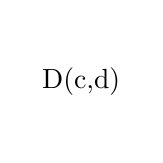
\begin{tikzpicture}[every node/.style={circle, minimum size=8mm}, level/.style={sibling distance=40mm/#1}, level distance=20mm]
                \node {D(c,d)};
            \end{tikzpicture}

            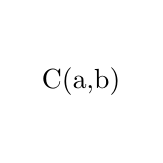
\begin{tikzpicture}[every node/.style={circle, minimum size=8mm}, level/.style={sibling distance=40mm/#1}, level distance=20mm]
                \node {C(a,b)};
            \end{tikzpicture}

            \begin{tikzpicture}[every node/.style={circle, minimum size=8mm}, level/.style={sibling distance=40mm/#1}, level distance=20mm]
                \node {B(a, b, c, d)}
                    child {node {C(a,b)}}
                    child {node {D(c,d)}};
            \end{tikzpicture}

            \begin{tikzpicture}[every node/.style={circle, minimum size=8mm}, level/.style={sibling distance=40mm/#1}, level distance=25mm]
                \node {A(b, d)}
                    child {node {B(a, b, c, d)}
                    child {node {C(a,b)}}
                    child {node {D(c,d)}}};
                    
            \end{tikzpicture}

            The proof tree for $A(b,d)$ already contains proofs for all the other elements of the program so that it would be enough to check this single tree.
        \end{example}

        We can define an element member function for trees in the usual way:

        \begin{lstlisting}
            def elementMember (a: A) (t: tree A): Bool  :=
            match t with
            | tree.node a' l => (a=a') ∨
             List.any l.attach (fun ⟨x, _h⟩ => elementMember a x)
        \end{lstlisting}
        In order for a tree to be valid all subtrees must be valid. A ground atom $ga$ is exactly then a member of a tree $t$ if there is a subtree of $t$ of which $ga$ is the root, so that if a proof tree is valid all elements are a subset of the semantics.

        \begin{lstlisting}
            lemma allTreeElementsOfValidTreeInSemantics 
            (t: proofTree τ)  (P: program τ) (d: database τ) 
            (valid: isValid P d t)(ga:groundAtom τ)(mem: elementMember ga t):
             ga ∈ proofTheoreticSemantics P d :=
        \end{lstlisting}

        This allows us to establish the alternative property of \texttt{validateTreeList}

        \begin{lstlisting}
            lemma validateTreeListUnitIffSubsetSemanticsAndAllElementsHaveValidTrees 
            (P: List (rule τ)) (d: database τ) (l: List (proofTree τ)) 
            (ruleToString: rule τ → String) : validateTreeList P d l  ruleToString = Except.ok () ↔
            {ga: groundAtom τ| ∃ (t: proofTree τ), t ∈ l ∧ elementMember ga t } ⊆ proofTheoreticSemantics P.toFinset d 
            ∧ ∀ (t: proofTree τ), t ∈ l → isValid P.toFinset d t
        \end{lstlisting}

        Now it is enough to pass just one proof tree from our example to validate the whole input and use in general less trees. 

        \subsection{Graph validation}

        We have finished the last section with a method to check whether a result is a subset of the semantics. For this we need a list of trees representing the result set. Finding such a list is however difficult. Viewing a tree as a set of its elements we see that it is an instance of the NP-hard set cover problem. Additionally, we found in practice that the datalog reasoner we used did only return a list of derivations. Constructing trees from this turned out to be computationally expensive, but the output can be interpreted as a directly acyclic graph. In the following section we describe how to validate such a graph.

        A number of different results of graph theory are already proven in mathlib. Nonetheless, we defined our own graph model in Lean for this section due to two main reasons. Firstly, the graph defined in mathlib is a undirected graph, but we require a directed graph so that we can see for a vertex (which represents a ground atom) which neighbors were used to derive it and which neighbors were derived from it. Secondly, the graph represents the edge relation as a map to \texttt{Prop} which is in general not computable.


        Our graph model consists of a list of vertices and a function that maps to each element the list of its predecessors. Representing the vertices as a list allows us to iterate over all vertices when validating the graph. We used a function to the predecessors instead of a adjancency matrix similar to the definition in mathlib in order to directly get the predecessors to a node instead of having the iterate over all vertices and check the adjancency matrix. This approach does have a small drawback. Suppose we want to determine whether a property holds for every vertex and do this by exploring the graph using depth-first search and we find a counterexample by following the predecessors. Nothing states that this vertex is actually in the graph, i.e. the list of vertices. This is an undesireable property so that we additionally ask for a proof that the predecessors of every vertex are again vertices in the graph.

        \begin{lstlisting}
            structure Graph (A: Type) where
                (vertices: List A)
                (predecessors: A → List A)
                (complete: ∀ (a:A), a ∈ vertices →  
                ∀ (a':A), a' ∈ predecessors a → a' ∈ vertices)
        \end{lstlisting}
        
        A standard definition of graph theory are walks as a sequence of connected edges. As we do not have edges directly, we represent this as a list of elements with two properties. A list of elements is a walk in a graph, if all elements are a vertices of the graphs and neighboring vertices are connected via the the predecessor relation of the graph. Due to the completeness property of the graph it would also be sufficient to express that the last element of the path is in the graph. 

        \begin{lstlisting}
            def isWalk (l: List A) (G: Graph A): Prop :=
            ( ∀ (a:A), a ∈ l → a ∈ G.vertices ) 
            ∧ ∀ (i: ℕ), i > 0 → ∀ (g: i < l.length), 
            l.get (Fin.mk i.pred (pred_lt i l.length g)) ∈ 
             G.predecessors (l.get (Fin.mk i g) )
        \end{lstlisting}

        We note that we do allow empty paths. This simplifies some proofs and algorithms even if there is no direct equivalent in graph theory. We specifically use lists as we are going to expand walks at the front when exploring the graph.  
        
        \begin{lemma}
            Let $w$ be a walk in a graph $G$ of the form $a::tl$. Then also $b::a::tl$ is a walk in $G$ for every predecessor $b$ of $a$.
        \end{lemma}

        Using walks we can define cycles. Every cycle is a walk. Additionally we require that it the start and the end of the walk are equal. In order to have a start and end we have to exclude the empty walks. Additionally, we exclude walks of a single element. Allowing them as cycles would mean that there are no acyclic graphs.

        \begin{lstlisting}
            def isCycle (l: List A) (G: Graph A): Prop :=
            if h: l.length < 2
            then False
            else
                have l_not_zero: 0 < l.length :=
                by
                cases ll: l.length with
                | zero =>
                    rw [ll] at h
                    simp at h
                | succ n =>
                    simp

                isWalk l G ∧
                 l.get (Fin.mk 0 l_not_zero) 
                 = l.get (Fin.mk l.length.pred (Nat.pred_lt (Ne.symm (Nat.ne_of_lt l_not_zero))))
        \end{lstlisting}

        A graph is then acyclic if no list represents a cycle in it.

        \begin{lstlisting}
            def isAcyclic (G: Graph A) := ∀ (l: List A), ¬ isCycle l G
        \end{lstlisting}

        We need to check whether a given graph is acyclic as only those graphs represent valid derivations. A cycle would mean that we used an atom to derivate itself and we could not get a valid proof tree for this element. We are going to use depth-first search to check whether a graph is acyclic. For this we need an alternative characterization of acyclicity.
        A first candidate for this would be the membership in a cycle.

        \begin{lemma}
            A graph is acyclic iff no vertice is a member in a cycle.
        \end{lemma}

        Ideally, we want this characterization to be an iff connection between a vertice and its predecessors. Unfortunately the statement does not hold for this characterization.

        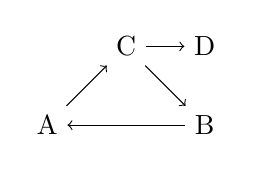
\begin{tikzpicture}
            \node (A) at (0,0) {A};
            \node (B) at (2,0) {B};
            \node (C) at (1,1) {C};
            \node (D) at (2,1) {D};
        
            \draw[->] (B) -- (A);
            \draw[->] (C) -- (B);
            \draw[->] (A) -- (C);
            \draw[->] (C) -- (D);
        \end{tikzpicture}

        D is not a member in a cycle, but its predecessor C is, so that an iff does not hold. Instead we see that D can be reached from a cycle using some walk. If it can be reached from a cycle, then also one of its predecessors can be reached from a cycle. We are going to formalize this idea in the following lemmas.

        Let $a$ and $b$ be two nodes. We say that $a$ can reach $b$ in $G$ if there exists a walk in $G$ that starts with $a$ and ends with $b$.

        \begin{lstlisting}
            def canReach (a b: A) (G: Graph A):= ∃ (w: List A) (neq: w ≠ []),
            isWalk w G ∧
            w.get (Fin.mk 0 (getFirstForNonequal_isLt w neq)) = a ∧
            w.get (Fin.mk w.length.pred (getLastForNonequal_isLt w neq)) = b
        \end{lstlisting}

        A singleton path allows us to show that any element can reach it self. Additionally, if $a$ can reach $b$ and $b$ is a predecessor of $c$ we can extend the path from $a$ to $b$ with $c$ in order to demonstrate that $a$ can reach $c$. Using the \texttt{canReach} predicate we can now express a different characterization for acyclicity, being reachable from a cycle. A node $a$ is reachable from a cycle $c$, if there exists a node $b$ in the cycle that reaches $a$. In the previous example $D$ is reached from a cycle as $C$ is in a cycle and $C$ reaches $D$. The same holds for $C$ as $C$ reaches itself.

        \begin{lstlisting}
            def reachedFromCycle (a:A) (G: Graph A):=
             ∃ (c: List A), isCycle c G ∧ ∃ (b: A), b ∈ c ∧ canReach b a G
        \end{lstlisting}

        \begin{lemma}
            A graph $G$ is acyclic iff all vertices of $G$ are not reached from a cycle.
        \end{lemma}
        \begin{proof}
            If $G$ is acyclic, then showing that all vertices of $G$ are not reached from a cycle is equivalent to showing that any cycle in $G$ cannot reach any element. Due to the acyclicity we know that no cycles exist in G so that the first direction is shown.

            The back direction is proved via contradiction. Assuming that the graph is not acyclic, we know that there must exist a cycle $c$ in $G$. Cycles in $G$ are nonempty lists of vertices that are all in $G$. As any vertex can reach itself, there are vertices that are reached from a cycle in contrast to our assumption, so that we have reached the contradiction.
        \end{proof}

        \begin{lemma}
            A node $a$ is not reached from a cycle iff all predecessors $b$ are not reached from a cycle.
        \end{lemma}
        \begin{proof}
            Both directions are proven via contradiction. For the first we have that there is a predecessor $b$ of $a$ that is reached from a cycle. Then we can simply extend the path by adding $a$ and then $a$ would be reached from a cycle.

            For the backdirection we assume that $a$ is reached from a cycle and try to show then one of its predecessors must also be reached from a cycle. 
            If $a$ is reached from a cycle $c$ with an element $b$ we consider two cases. 
            If $b$ would be a predecessor, then we have reached a contradiction as $b$ is in the circle and reaches itself. Now we assume that $b$ is not a predecessor of $a$. Again we can consider two cases. If the path is of length one then $a$ and $b$ must be equal and $a$ is a member in a cycle. As long as $a$ is not the first element in the cycle, we can simply pick the preceeding element in the cycle due to the connectness property of the walk. This does not work if $a$ is the first element, but since it is a cycle $a$ must also be the last element and we can pick the predecessor of the last element, which is a predecessor of $a$ and in a cycle.

            If $a$ is reached from a path longer than length 1, we simply pick the subpath without the last element. This is not empty and ends with a predecessor of $a$, which is therefore reached by a cycle. In every case we reached a contradiction so that the claim must be true.
        \end{proof}

        This completes a characterization of acyclicity that has an iff relation between a node and its predecessors. We still need a method to detect a cycle. We are going to explore the graph via walks and add the current element to the walk whenever we reach a new node. If we see a node again, we have reached a cycle.

        \begin{lemma}
            Let $w$ be a walk in a graph $G$ and $a$ be a node of $G$ so that $a::w$ is also a walk in $G$. If $a$ is a member of $w$, then there exists a cycle in $G$.
        \end{lemma}

        For this we need to extract the walk from $a$ to $a$ out of $a::w$. This is done by the \texttt{getSubListToMember} function. We are given an element $a$, a list $l$ and a proof of $a\in l$ and want to return the sub list until $a$. This is defined inductively. The empty case of $l$ is impossible as $a$ can be a member of the empty list. In the cons case we keep the head element of the list in the result. If this is already $a$, then we stop, else $a$ must be a member in the tail and we continue.

        \begin{lstlisting}
            def getSubListToMember (l: List A) (a: A) (mem: a ∈ l): List A :=
            match l with
            | [] =>
                have h: False :=
                by
                simp at mem

                False.elim h
            | hd::tl =>
                if p: a = hd
                then [hd]
                else
                have mem': a ∈ tl :=
                by
                    simp[p] at mem
                    apply mem
                hd::getSubListToMember tl a mem'
        \end{lstlisting}

        In any case the list is never empty as we return at least the head of the list we called \texttt{getSubListToMember} on and in both cases the resulting list $l'$ starts with the same element as $l$ used to. By calling it on $w$ with the member $a$ the result $l'$ starts with the same element as $w$. Since $a::w$ was a walk, we therefore can also extend $l'$ with $a$ and preserve a walk assuming that $l'$ preserves a walk. This can be proven by induction. If we have reached the element we return a list with a single element that is a member of $G$, which is always a walk. If not we keep the element and add this to the result of \texttt{getSubListToMember} on the tail. This result is by the induction hypothesis a walk and by the previous result keeps the first element so that we can attach $hd$ again to the front and get a walk. Now we now that the result of \texttt{getSubListToMember a w mem} is a walk and that also \texttt{a::(getSubListToMember a w mem)} is walk. 
        In order to show that this a cycle we need two more facts. Firstly, this list should have a length of at least two. This is the case as \texttt{getSubListToMember} never returns an empty list, so that it has at least length one and also attaching $a$ to the front increases the length by one. Secondly, we need the resulting list of \texttt{getSubListToMember a w mem} to end with $a$ so that \texttt{a::(getSubListToMember a w mem)} is cycle. This can again be proven by induction, since the list only ends when $a$ is encountered. 

        These facts are enough to start implementing and proving depth-first search in order to check whether the given graph is acyclic. This is however not the only criteria necessary for a valid derivation graph. Additionally, we have to check all steps are valid according to the program as well. We could check this separately, but we will visit all vertices of the graph during the execution of depth first search anyway, so that combining these steps seems more efficient. 

        We generalize this by defining depth-first search with a function that takes a vertex and a list of vertices representing the predecessors that is evaluated during the search. We need again a criteria that the depth-first search shall fulfill if it returns acceptance. As we explore the graph want depth-first search to return ok on a vertex $a$ if all vertices reachable from $a$ return ok on the function with their predecessors.

        \begin{lemma}
            Let $f:$ \texttt{A → List A → Except String Unit} be a function and $G$ a graph. Then $f$ returns ok for all vertices and their predecessors iff $f$ returns ok for all vertices that can reach a vertex in $G$. 
        \end{lemma}
        \begin{proof}
            $\Rightarrow$: Any vertex that can reach $a$ in $G$ must also be in $G$. By the assumption therefore $f$ is evaluated to ok on this vertex and its predecessors.

            $\Leftarrow$: As any vertex can reach itself all vertices must return ok when evaluating $f$ with their predecessors.
        \end{proof}

        Additionally, we see that for every node $a$ all nodes that reach $a$ either reach a predecessor of $a$ or are $a$ themselves.

        Now we can define our depth-first search algorithm. In general we follow the definition in \cite{AlgorithmsBook}, but use some helper functions in order to simplify the proofs. Similar to the book we use two main function. A first function \texttt{dfs} calls on all vertices the \texttt{dfs\_step} function that explores graph that can reach this node. In order to not explore a vertex multiple times we return a set of nodes that were already explored. For this we originally used \texttt{Finset} but this turned out to be not fast enough in practice, so that we changed to \texttt{HashSets}.

        The function \texttt{addElementIfOk} takes an exception of type \texttt{B} and \texttt{HashSet}. If this exception is ok, i.e. a \texttt{HashSet} it inserts the given element into the hash set. If the exception is an error, we simply return the exception.

        \begin{lstlisting}
            def addElementIfOk [Hashable A] (e: Except B (HashSet A)) (a:A):
             Except B (HashSet A) :=
            match e with
            | Except.ok S => Except.ok (S.insert a)
            | Except.error msg => Except.error msg
        \end{lstlisting}

        From the definition we see that \texttt{addElementIfOk} returns a hash set iff the original exception was already a hash set.

        As we are going to call \texttt{dfs\_step} on all predecessors, we use \texttt{foldl} to not explore a vertex multiple times. Our version is a bit modified in order to work with the exceptions. If an error is detected, we stop.

        \begin{lstlisting}
            def foldl_except_set [Hashable B] 
            (f: A → HashSet B → (Except String (HashSet B)))
             (l: List A) (init: HashSet B):
              Except String (HashSet B) :=
            match l with
            | [] => Except.ok init
            | hd::tl =>
                match f hd init with
                | Except.error msg => Except.error msg
                | Except.ok S => foldl_except_set f tl S

        \end{lstlisting}

        The \texttt{dfs\_step} function is called on a vertex $a$ in the graph $G$ together with a function $f$ that shall be evaluated on every vertex and its predecessors in $G$. Additionally, we receive a set \texttt{visited} that contains all explored vertices and the walk \texttt{currWalk} we used in the graph to arrive at the current vertex $a$. In order to prove termination it is important that also \texttt{a::currWalk} is a walk again and that $a$ is not a member of \texttt{currWalk}. As we recursively call \texttt{dfs\_step} we extend the walk by the current node and argue that the number of nodes that are not in the walk decreases. This only works if $a$ is not already present in the walk.

        The procedure starts by checking whether the current node is already explored, i.e. \texttt{visited} contains it. If that is the case, we simply return \texttt{visited} and are done. If not we have to explore the graph. Firstly, we check if $f$ is evaluated on the current node and its predecessor to ok. If this is not the case, we have found a counterexample. If it is evaluated to ok, then we check if any predecessor of $a$ is equal to $a$ or in the current walk. This would imply the existance of a cycle and we would report this as an error. 
        Finally we call \texttt{dfs\_step} on every predecessor and use \texttt{foldl\_except\_set} to not explore vertices twice. If this returns a hash set, then we add the current node to it. 


        \begin{lstlisting}
            def dfs_step [Hashable A] (a: A) (G: Graph A) 
            (f: A → List A → Except String Unit) 
            (currWalk: List A) (walk: isWalk (a::currWalk) G) 
            (not_mem: ¬ (a ∈ currWalk))(visited: HashSet A) :
             Except String (HashSet A) :=
            if visited.contains a
            then Except.ok visited
            else
                match f a (G.predecessors a) with
                | Except.error msg => Except.error msg
                | Except.ok _ =>
                if pred_walk: (G.predecessors a) ∩ (a::currWalk) = []
                then

                addElementIfOk (foldl_except_set (fun ⟨x, _h⟩ S =>
                    dfs_step x G f (a::currWalk) 
                     (isWalk_extends_predecessors walk x _h) 
                      (not_mem_of_empty_intersection pred_walk x _h) S) 
                    (G.predecessors a).attach visited
                ) a
                else
                    Except.error "Cycle detected"
        \end{lstlisting}


        The desired property of \texttt{dfs\_step} is the following lemma.

        \begin{lemma}\label{lem:dfsstep}
            Let $a$ be a vertex and $S$ be a set such that any member $a'$ of $S$ is not reached from a cycle and that any vertex $b$ that reaches $a'$ is evaluated to \texttt{ok} on $f$. Then \texttt{dfs\_step a G f walk currWalk walk not\_mem S} is evaluated to \texttt{ok} iff $a$ is not reached from a cycle and all vertices $b$ that reach $a$ are evaluated on $f$ with their predecessors to \texttt{ok}.
        \end{lemma}

        For this we need to determine whether \texttt{foldl\_except\_set} returns an exception or not, which seems dauting due to chaining of results. We get a result for the first predecessors and use this to evaluate the second predecessors and so on and it seemed difficult to determine when its wrong and why. We need this function however to not explore vertices multiple times. This set of previously explored nodes is semantically not so important. We could also work always with the empty set and get the same result with more effort. It only becomes problematic if the set contains elements that are reached from a cycle or an element for which $f$ is not evaluated to ok. We generalize this by considering a property $p$ of vertices and call a function $g$ independent from $p$, if for any node $a$ and sets $S, S'$ whose member both all satisfy $p$, $g( a, S)$ is ok iff $g( a S')$ is ok. This is pretty close to allowing us to consider it as separate calls instead of chaining the results. Additionally we need that $g$ also preserves $p$, i.e. when $S$ is a set whose members all satisfy $p$, then all members of the result $S' = g(a,S)$ also satisfy $p$. Then the initial set can be used instead of the result as both sets only have members that satisfy $p$ and are with respect towards the kind of exception equivalent. Therefore we gain the following lemma by induction to determine the kind of exception of \texttt{foldl\_except\_set}.

        \begin{lemma}\label{lem:fes_ok}
            Let $g: A \to HashSet B \to Except String (HashSet B)$ be a function that is independent from a property $p: A \to Prop$ and that preserves $p$. Then for any list $l$ and any hash set $init$ whose members all satisfy $p$, \texttt{foldl\_except\_set} $g$ $l$ $init$ is ok iff $g a init$ is ok for all elements $a$ from $l$.
        \end{lemma}

        The function $g$ shall represent \texttt{dfs\_step} on the predecessors of a vertex $a$ and $p$ be that a vertex is not reached from a cycle and all elements that reach this vertex are evaluated as ok under $f$. From the induction hypothesis of \ref{lem:dfsstep} we will get the independence from $p$ as the statement of the lemma does not depend on the HashSet at all. Seperatedly we need to prove that \texttt{dfs\_step} preserves the above defined property $p$. The previous lemmas combined the value of for our $p$ on a vertex $a$ with the value of $p$ on $a$'s predecessors. Therefore we want to prove that the resulting set of \texttt{foldl\_except\_set} on the predecessors contains all predecessors and all its members satisfy $p$ in order to conclude that the node $a$ we started from satisfies $p$.

        For this we will prove that \texttt{dfs\_step} always returns a subset of the input when it returns ok and need the following lemma for \texttt{foldl\_except\_set}, which can be proven by induction
        \begin{lemma}
            Let $g: A \to HashSet B \to Except C (HashSet B)$ be a function so that for all $a$ and $S, S'$, if $g(a,S) = ok S'$, then $S \subseteq S'$. Then also for any list $l$ and sets $S, S'$ with \texttt{foldl\_except\_set} $l$ $S S'$ we have that $S \subseteq S'$.
        \end{lemma}

        Now we can prove the claim for \texttt{dfs\_step}. The induction for \texttt{dfs\_step} will follow the same structure with the unsatisfiable start and will later be omitted.

        \begin{lemma}
            If \texttt{dfs\_step a G f walk currWalk walk not\_mem S} returns a set $S'$, then we have $S \subseteq S'$.
        \end{lemma}
        \begin{proof}
            We prove this by induction on the number of uncovered vertices by the current path. In the induction basis any vertex is already in the path yet \texttt{not\_mem} tells us that $a$ is not a member in the path, which is a contradiction.
            In the step we do a case distinction whether $a$ is already contained in $S$. If that is the case, then $S$ is returned and due to the reflexivity the claim is proven.
            If not we return the result of a insertion into the result of \texttt{foldl\_except\_set} so that it is sufficient to show that \texttt{foldl\_except\_set} returns a superset of $S$. This is done by the previous lemma together with the induction hypothesis as the path is longer so a smaller amount of vertices is not covered by the path.
        \end{proof}

        We know that \texttt{dfs\_step} returns a superset of the input set, but what elements are added to this set ? That are essentially all nodes that can reach the node we started our search step from assuming that the visited set already fulfills this property. This theorem is more complicated and for our goals it suffices to know that the starting node is added to the result set assuming it is returned.

        \begin{lemma}
            If \texttt{dfs\_step a G f walk currWalk walk not\_mem S} returns a set $S'$ then $S'$ contains $a$.
        \end{lemma}
        \begin{proof}
            This is proven by case distinction. If $a$ is already contained in $S$, then $S$ is returned and by that the claim is proven.

            If $a$ is not contained in $S$, then the resulting set $S'$ is obtained by inserting $a$ into the resulting set of \texttt{foldl\_except\_set}, so that due to properties of insert $a$ is a member of $S'$.
        \end{proof}
        

        Using these two results we have a criteria to show when \texttt{foldl\_except\_set} contains the original list. Due to Lean internal features, the result must be a bit more technical. As we need to show termination in order to unfold our function, we call \texttt{foldl\_except\_set} not on the predecessors of $a$, but instead of the attached version of this list, which is a different type. Therefore we use a function mapping the list type to the set type and refer to the result of this function as the mapped form.

        \begin{lemma}
            Let \texttt{f: A → HashSet B → (Except String (HashSet B))} and {g: A → B} be functions such if $f(a,S) $ returns a hash set $S'$  then $S \subseteq S'$ and $g(a) \in S'$. Then for any list $l$ and hash set S,  if \texttt{foldl\_except\_set f l S} returns a hash set $S'$, then for all elements $a$ of $l$, $g(a) \in l$.
        \end{lemma}
        \begin{proof}
            We prove this by induction on $l$.
            If $l$ is empty all elements of $l$ are in their mapped form in the resulting set.

            If $l$ has the shape $hd::tl$, then we first compute $f(hd,S)$ which must return a set $S'$ since the whole function returns a set. $S'$ must contain $g(hd)$ and is passed into \texttt{foldl\_except\_set} which by the induction hypothesis contains all elements of $tl$ in their mapped form. Due to the subset property all elements of $S'$ must also be contained, so that also $g(hd)$ is in the result. Therefore all elements of the list are contained in their mapped form in the resulting set, if it exists.
        \end{proof}

        This allows us to show that \texttt{dfs\_step} preserves our property $p$, that is that a vertex $a$ is not reached from a cycle and all vertices that reach $a$ are together with their predecessors evaluated to ok by $f$. For shortness we call this again the property $p$ in the following lemma.

        \begin{lemma}
            If \texttt{dfs\_step a G f walk currWalk walk not\_mem S} returns a set $S'$ and all elements in $S$ have the property $p$, then also all elements in $S'$ have the property $p$.
        \end{lemma}
        \begin{proof}
            This is again proven by the number of vertices not covered by the current walk. 

            In the step we must consider again two cases. If $a$ is already a member of $S$, then $S$ is returned and all elements of $S$ fulfill the property $p$ by assumption. If not then $f(a, G.predecessors(a))$ must be ok. Additionally, \texttt{foldl\_except\_set} must return a hash set $S'$ calling \texttt{dfs\_step} on the predecessors of $a$, which all don't occur in currWalk. Therefore the number of uncovered nodes is smaller, we from the induction hypothesis we know that all these function preserve $p$ and by a separate induction argument also \texttt{foldl\_except\_set} preserves then $p$. The returned hash set is then \texttt{S'.insert a}. As all elements of $S'$ satisfy $p$, we must show that also $a$ satisfies $p$. We know that all predecessors of $a$ are in $S'$.  Firstly, we see that all predecessors of $a$ are in $S'$ and therefore not reached from a cycle, so that also $a$ is not reached from a cycle. Secondly, all elements that reach a predecessor of $a$ fulfill $f$ with their predecessors and also $a$ fulfills $f$ with its predecessors so that $a$ also satisfies $p$.
        \end{proof}

        Now we have the required tools to finally prove the main lemma \ref{lem:dfsstep} if \texttt{dfs\_step} and do this again by induction.
        
        In the induction step we show both direction seperatedly. First we assume that \texttt{dfs\_step a G f walk currWalk walk not\_mem S} returns a set $S'$. We know that $S$ already had the property $p$ and therefore also $S'$ has the property $p$, which is directly the other direction. Therefore it is enough to show that $a$ is contained in $S'$, which we have already shown.

        For the other direction we know that $a$ is not reached from a cycle and all elements that reach $a$ satisfy $f$ and want to show that \texttt{dfs\_step} returns ok. If $a$ is in $S$, then this is the case, so we consider the case of $a$ not contained in $S$. As $a$ can reach itself, $f(a, G.predecessors(a))$ must be ok. Also none of the predecessors of $a$ can occur in the current walk as the would imply a cycle that can reach $a$ in contrast to our assumption. The result is now the result of \texttt{addElementIfOk} which is ok iff the original exception was ok. The original exception is the result of \texttt{foldl\_except\_set}. For this we apply \ref{lem:fes_ok}. The preservation of $p$ was proven before and from the induction hypothesis we see that \texttt{dfs\_step} is independent from $p$, as it being ok does not depend on the set. Additionally, we have to show that all predecessors of $a$ are evaluated to ok on \texttt{dfs\_step}. Using the induction hypothesis this is equivalent to showing that all predecessors are not reached from a cycle and all elements that reach them are evaluated to ok which follows from the assumption. This ends the proof as we have shown both directions.

        We have shown the correctness of \texttt{dfs\_step} where we explore all vertices that can reach the start vertices. In order to fully explore the graph, we call this function on every vertex. By using \texttt{foldl\_except\_set} we keep track of the visited vertices, so that we simply return when we already encountered a vertex. 

        At the end we do not care anymore about the resulting set and only whether it was ok or if not the error message for which we use the following function for easier proofs. This functions returns ok iff the original returned some element with ok.

        \begin{lstlisting}
            def isOkOrMessage (e: Except String A): Except String Unit :=
            match e with
            | Except.error msg => Except.error msg
            | Except.ok _ => Except.ok ()

            def dfs [Hashable A] (G: Graph A) 
            (f: A → List A → Except String Unit) :
             Except String Unit :=
  
            isOkOrMessage (foldl_except_set 
             (fun ⟨x,_h⟩ S => dfs_step x G f [] (isWalkSingleton G x _h) 
               (List.not_mem_nil x) S)
              G.vertices.attach HashSet.empty 
            )
        \end{lstlisting}

        This shall return ok iff the graph is acyclic and all its vertices are evaluated to ok with respect to the input function and their predecessors.

        \begin{lemma}
            \texttt{dfs G f} returns ok iff $G$ is acyclic and for all vertices $a$ of $G$, $f(a, G.predecessors(a))$ is evaluated to ok.
        \end{lemma}
        \begin{proof}
            Due to the property of \texttt{isOkOrMessage}, we can replace the left side simply by the \texttt{foldl\_except\_set} on \texttt{dfs\_step}. We know that \texttt{foldl\_except\_set} is ok iff calling \texttt{dfs\_step} on every node with the empty set, which fulfills $p$, returns ok. The prerequisites are fulfilled, because we have proven that \texttt{dfs\_step} preserves $p$ and is independent from $p$ by the semantics lemma. Therefore this is ok, if all vertices of the graph are not reached from a cycle and any vertex reaching a vertex evaluates $f$ to ok with their predecessors. This is equivalent to being acyclic and evaluating $f$ returns ok for any vertex and its predecessors.
        \end{proof}

        We have designed the depth-first search algorithm to evaluate a function during the search. This function shall inform us that the graph encodes a datalog derivation. This function shall check only a vertex and its predecessors encode a valid datalog derivation, so that we call the property locally valid. This is very similar to the definition of \texttt{isValid} for trees except for the missing \texttt{List.All₂}.

        \begin{lstlisting}
            def locallyValid (P: program τ) (d: database τ) (v: groundAtom τ) 
            (G: Graph (groundAtom τ)): Prop :=
            (∃(r: rule τ) (g:grounding τ), r ∈ P 
            ∧ ruleGrounding r g = groundRuleFromAtoms v (G.predecessors v) ) 
            ∨ ((G.predecessors v) = [] ∧ d.contains v)
        \end{lstlisting}

        The function checking this criteria is again very similar to the one we defined earlier for trees and by a similar argument we show that it is a checker for being locally valid.

        \begin{lstlisting}
            def locallyValidityChecker (m: List τ.relationSymbols → List (rule τ))
            (d: database τ) (l: List (groundAtom τ))
            (a: groundAtom τ): Except String Unit :=
            if l.isEmpty
            then
                if d.contains a
                then Except.ok ()
                else checkRuleMatch m (groundRule.mk a l) 
            else
                checkRuleMatch m (groundRule.mk a l)
        \end{lstlisting}

        \begin{lemma}
            Let $d$ be a database and $a$ a ground atom, that is a vertex in a graph $G$.
            If we use as $m$ the result of \texttt{parseProgramToSymbolSequenceMap} for a program $P$, then \texttt{locallyValidityChecker m d (G.predecessors a) a} returns \texttt{ok} iff $a$ is locally valid in $G$ for $d$ and $P$.
        \end{lemma}

        Next, we need to use an acyclic graph where all vertices are locally valid to obtain virtual proof trees to show that the vertices are part of the proof-theoretic semantics of datalog. This is done by a function that is similar to depth-first search so that we could reuse its termination argument. The acyclicity of the graph offers us though a different termination argument that simplifies some proofs later.

        We already introduced the \texttt{canReach} predicate. All vertices that can reach a vertex $a$ are in some sense a predecessor of $a$. We call all these elements the \textit{global predecessors of $a$}. As any graph is finite and any element that can reach an element in a graph must also be in the same graph, the global predecessors form a finite set. We would like to use the \texttt{Finset.filter} function to gain the predecessors from the finite set of the vertices of a graph. Unfortunately, \texttt{canReach} is not decidable itself (though we can use depth-first search to decide it), which is required to use \texttt{Finset.filter}. Therefore we define an own version of \texttt{Finset.filter} that accepts also by using the original \texttt{Finset.filter} function with the result that any predicate is classically decidable.

        \begin{lstlisting}
            noncomputable def Finset.filter_nc (p: A → Prop) (S: Finset A):= 
            @Finset.filter A p (Classical.decPred p) S
        \end{lstlisting}

        Using classical logic we can also reproof a membership lemma for \texttt{Finset.filter} from mathlib.

        \begin{lemma}
            Let $S$ be a finite set and $p$ a predicate and $S'$ be the result of \texttt{Finset.filter\_nc p S}. Then any element is a member in $S'$ iff it is a member of $S$ and $p$.
        \end{lemma}

        Using this filter allows us to define the global predecessor formally.

        \begin{lstlisting}
            noncomputable def globalPredecessors (b:A)(G: Graph A):Finset A:=
            Finset.filter_nc (fun a => canReach a b G) G.vertices.toFinset
        \end{lstlisting}

        In order to show termination we will need that the global predecessors of a predecessor of $a$ is a strict subset of the predecessors of $a$. Therefore the cardinality of the set of the global predecessors decreases and the algorithm will terminate.

        \begin{lemma}
            Let $a$ be a vertex in a graph $G$ and $b$ a predecessor of $a$. Then \texttt{globalPredecessors b G} $\subseteq$ \texttt{globalPredecessors a G}
        \end{lemma}
        \begin{proof}
            Any element $c$ in \texttt{globalPredecessors b G} has a walk $w$ that ends with $b$. Since $b$ is a predecessor of $a$, $w++[a]$ is also a walk and therefore $c$ also reaches $a$ and is therefore in the global predecessors of $a$. 
        \end{proof}

        \begin{lemma}
            Let $a$ be a vertex in an acyclic graph $G$ and $b$ a predecessor of $a$.
            Then $a$ is not in the global predecessors of $b$.
        \end{lemma}
        \begin{proof}
            Suppose that $a$ would be in the global predecessors of $b$. Then we would have a walk $w$ from $a$ to $b$ that has a length of at least one. Then we can again obtain the walk $w++[a]$ that has at least length two and starts and ends with $a$. This would be a cycle in $G$ in contrast to our assumption that $G$ is acyclic. Therefore $a$ can not be a member of the global predecessors of $b$.
        \end{proof}

        These results suffice the show the termination for the next function. We form a tree by simply taking the current vertex as the root and use the result of all predecessors for the sub trees.

        \begin{lstlisting}
            def extractTree (a:A) (G: Graph A) 
            (mem: a ∈ G.vertices) (acyclic: isAcyclic G): tree A :=

            tree.node a (List.map 
            (fun ⟨x, _h⟩ => extractTree x G (G.complete a mem x _h) acyclic) 
            (G.predecessors a).attach)
        \end{lstlisting}

        The root of the tree that results from \texttt{extractTree a G mem acyclic} is obviously $a$. If we extract for a ground atom $a$ in a graph where any vertex is locally valid, we gain a valid proof tree.

        \begin{lemma}
            Let $G$ be a graph of ground atoms, $P$ a program, $d$ a database and $a$ member of $G$. If all vertices of $G$ are locally valid and $G$ is acyclic, then $a$ has a valid proof tree for $P$ and $d$.
        \end{lemma}
        \begin{proof}
            We proof this by strong induction on the cardinality of the global predecessors for arbitrary $a$. As $a$ is a vertex in $G$ it is locally valid. There are two cases for this.

            We first consider the rule case, i.e. $a$ and its predecessors are an instance of a ground rule from $ground(P)$. We can reuse this rule as the roots of the subtrees are the same as the predecessors of $a$ by our previous assumption. Additionally, all direct subtrees are valid as well by our induction hypothesis. Due to the acyclicity of the graph, the global predecessors of any predecessor $b$ of $a$ form a strict subset of the global predecessors of $a$, so that their cardinality is lower.

            The other option would be that $a$ has no predecessors and is in the database. Then \texttt{extractTree} will add no subtrees, so that the resulting tree is again valid.
        \end{proof}

        The previous lemma tells us that any vertex in a graph that is acyclic and has only locally valid vertices has a valid proof tree. Therefore the vertices of this graph form a subset of the proof-theoretic semantics and we use the graph validation as an alternative for the tree validation.



        

    \section{Completeness}

    In the previous chapter we described a method why an atom is in the datalog semantics. This criteria is however not sufficient to recognize a solution. The empty list passes this test for any program while not being the semantics in most cases. Proof trees were a method to recognize why a ground atom is part of the semantics, but we are not aware of any simple way to describe why a ground atom is not in the semantics. Instead we want to show that the set of elements in the proof trees, $S$ are complete in the sense that nothing else can derived from it any more. This is the case when the $T_P$ operator has a fixed-point for $S$ or alternatively when $S$ is a model. In this chapter we are going to create a certified model checker to show the completeness. If $S$ passed the tree validation algorithm and is a model the following statements hold:

    \[ S \subseteq \mathtt{proofTheoreticSemantics\ P\ d} = \mathtt{modelTheoreticSemantics\ P\ d} \subseteq S \]

    \subsection{Partial ground rules}
    
        We defined the model property on the ground program $ground(P)$. In order to check if a set of ground atoms is a model for a program we therefore have to ground the program. We want to avoid simply grounding all the rules at once and instead do it in a more intelligent way. For this we introduce a new data structure, the partial ground rule. This bears some similarities to the rules we defined in chapter 3. It has a head that is an atom. The body is split into two lists. The first list contains the ground atoms and represents the atoms in the rule we already grounded, whereas the second list consists of the so far ungrounded atoms in the rule body. We want to move the ungrounded atoms one by one into the grounded list by applying substitutions, which map all variables of this atom to constants, so that we can transform this atom into a ground atom.

        \begin{lstlisting}
            structure partialGroundRule (τ: signature)  where
                head: atom τ
                groundedBody: List (groundAtom τ)
                ungroundedBody: List (atom τ)
        \end{lstlisting}

        \begin{example}
            A rule $r := q(X) :- r(a, b), t(X, c), s(c, d), u(d, X) .$ may be viewed as the following partial ground rule
            $pgr_1 = $
            \begin{lstlisting}
                {
                    head:= q(X),
                    groundedBody := [],
                    ungroundedBody := [r(a, b), t(X, c), s(c, d), u(d, X)]
                }
            \end{lstlisting}
            
            This representation does not look any different to the rule itself as we do not use the grounded body at all. We can however move ground atoms from the ungrounded body into the grounded body. The order of the atoms in the body does not matter semantically as we use a set definition when defining the criteria for a rule being true, so that we can simply move all ground atoms in the grounded body.

            \begin{lstlisting}
                {
                    head:= q(X),
                    groundedBody := [r(a, b), s(c, d)],
                    ungroundedBody := [t(X, c),  u(d, X)]
                }
            \end{lstlisting}

        \end{example}

        We can transform any rule into a partial ground rule by setting the head as the head, the body as the ungrounded body and setting the grounded body to be empty.

        \begin{lstlisting}
            def partialGroundRuleFromRule (r: rule τ): partialGroundRule τ :=
            {
                head := r.head, 
                groundedBody := [],
                ungroundedBody := r.body
            }
        \end{lstlisting}

        \begin{example}
            $pgr_1$ is exactly the result of \texttt{partialGroundRuleFromRule $r$}.
        \end{example}

        We choose this representation instead of the approach used for $pgr_2$ as this does not require iterating over the whole body to find ground atoms. As we will apply multiple substitutions in the grounding process, we will create anyways ground atoms in different place to the atom in the body we are currently trying to ground.

        Any partial ground rule can also be transformed back into a rule by concatenating the grounded and ungrounded body and combining creating first a partial ground rule from a rule and then transforming the resulting partial ground rule yields the original rule. This does not hold if we swap the operations as we do not explicitly move atoms without variables from the start of the body into the grounded body.

        \begin{lstlisting}
            def partialGroundRule.toRule (pgr: partialGroundRule τ)
            : rule τ :=
    
            {
                head:= pgr.head, 
                body := (List.map (groundAtom.toAtom) pgr.groundedBody)
                ++ pgr.ungroundedBody
            }

            lemma partialGroundRuleToRuleInverseToFromRule (r: rule τ): 
                r = partialGroundRule.toRule (partialGroundRuleFromRule r)
        \end{lstlisting}

        \begin{example}
            The application of \texttt{partialGroundRule.toRule} on $pgr_1$ yields $r$ as predicted by the lemma.

            If we swap both functions and first apply \texttt{partialGroundRule.toRule} to a partial ground rule and then convert the resulting rule back to a partial ground rule, we see that this is no longer equal. Applying {partialGroundRule.toRule} to $pgr_2$ results in the rule $ q(X) :- r(a, b), s(c, d), t(X, c),  u(d, X) . $. Converting this back into a partial ground rule with \texttt{partialGroundRuleFromRule} we gain 

            \begin{lstlisting}
                {
                    head:= q(X),
                    groundedBody := [],
                    ungroundedBody := [r(a, b), s(c, d), t(X, c),  u(d, X)]
                }
            \end{lstlisting}
            which is different from $pgr_2$
        \end{example}

        Using the transformation to rules we can lift defintions like safety or being true to partial ground rules.

        \begin{lstlisting}
            def partialGroundRule.isSafe (pgr: partialGroundRule τ) :=
                pgr.toRule.isSafe

            def partialGroundRule.ruleTrue (pgr: partialGroundRule τ) 
            (i: interpretation τ) :=
                ruleTrue pgr.toRule i
        \end{lstlisting}

        So far we only split the body into two parts and have the goal of applying substitutions to move everything into the grounded body. This is not to different to just applying groundings directly. 
        This process allows us to potentially stop early. If the substitutions we applied so far resulted in a ground atom that is not part of the interpretation $i$ we already know that the rule is true. No matter how the remaining variables are mapped, the body will never be a part of $i$ and therefore the antecedent is false and the rule is therefore true. We call a partial ground rule \textit{active in an interpretation} $i$ where all ground atoms in the \texttt{groundedBody} 

        \begin{lstlisting}
            def active (pgr: partialGroundRule τ) (i: interpretation τ):=
            ∀ (ga: groundAtom τ), ga ∈ pgr.groundedBody → ga ∈ i 
        \end{lstlisting}

    \subsection{Explore grounding}

    \bibliography{main.bib}
    \bibliographystyle{plain}
\end{document}